% ============================================================
% PRM393 - OmniCast Mobile project report (Vietnamese version)
%
% Compile with:
%   xelatex main-vi.tex
%   xelatex main-vi.tex
% ============================================================
\documentclass[conference,a4paper]{IEEEtran}

% ============================================================
% OmniCast - Shared preamble for IEEEtran conference reports
%   PRN232 (VN / EN) and PRM393 (VN / EN)
% ============================================================

\newif\ifomniEN
\omniENfalse
\newcommand{\bi}[2]{\ifomniEN#2\else#1\fi}

% ---------- Fonts (Windows system fonts, full Vietnamese coverage) ----------
\usepackage{fontspec}
\setmainfont{Times New Roman}
\setsansfont{Arial}
\setmonofont{Consolas}
\XeTeXlinebreaklocale "vi"
\XeTeXlinebreakskip = 0pt plus 1pt

% ---------- Core packages ----------
\usepackage{amsmath}
\usepackage{amssymb}
\usepackage{booktabs}
\usepackage{multirow}
\usepackage{array}
\usepackage{graphicx}
\usepackage{xcolor}
\usepackage{enumitem}
\usepackage{tikz}
\usepackage{listings}
\usepackage{tabularx}
\usepackage{array}
\usepackage{url}
\usepackage{siunitx}
\usepackage[most]{tcolorbox}
\usepackage{fancyhdr}
\usepackage{lastpage}

% ---------- Page numbering & Running headers/footers ----------
\pagestyle{fancy}
\fancyhf{}
\setlength{\headheight}{14pt}
\renewcommand{\headrulewidth}{0.4pt}
\renewcommand{\footrulewidth}{0.4pt}
\fancyhead[L]{\footnotesize\textsf{\bi{OmniCast Mobile --- Báo Cáo Kỹ Thuật PRM393 (Mentor: Thầy Huỳnh Vang)}{OmniCast Mobile --- PRM393 Technical Report (Mentor: Mr. Huỳnh Vang)}}}
\fancyhead[R]{\footnotesize\textsf{\bi{Học Kỳ Fall 2026 (FA26)}{Fall 2026 Semester (FA26)}}}
\fancyfoot[L]{\footnotesize\textsf{FPTU Quy Nhon AI Campus --- FU Cahata}}
\fancyfoot[R]{\footnotesize\textsf{\textbf{\bi{Trang \thepage\ / \pageref{LastPage}}{Page \thepage\ of \pageref{LastPage}}}}}


\usetikzlibrary{positioning,arrows.meta,shapes.geometric,fit,backgrounds,calc,shadows,decorations.pathmorphing}

\usepackage{hyperref}
\pdfstringdefDisableCommands{%
  \ifomniEN\def\bi#1#2{#2}\else\def\bi#1#2{#1}\fi
}
\hypersetup{
  colorlinks=true,
  linkcolor=omniBlue,
  citecolor=omniTeal,
  urlcolor=omniPurple,
  pdftitle={OmniCast Mobile Project Report - PRM393},
  pdfauthor={Nguyen Binh An, Tran Thanh Son, Nguyen Vinh Phu, Dong Hoang Nguyen},
  pdfsubject={PRM393 - FPTU Quy Nhon AI Campus - FU Cahata},
  pdfkeywords={OmniCast, EPG, broadcast, LiveStream, Flutter, BLoC, FPTU Quy Nhon AI Campus, FU Cahata}
}

% ---------- OmniCast brand palette ----------
\definecolor{omniBlue}{HTML}{0E7490}
\definecolor{omniDark}{HTML}{0F172A}
\definecolor{omniTeal}{HTML}{0D9488}
\definecolor{omniPurple}{HTML}{7C3AED}
\definecolor{omniAmber}{HTML}{D97706}
\definecolor{omniRose}{HTML}{E11D48}
\definecolor{omniSlate}{HTML}{475569}
\definecolor{omniLight}{HTML}{F1F5F9}
\definecolor{omniBorder}{HTML}{CBD5E1}

% ---------- Typography tweaks ----------
\renewcommand{\familydefault}{\rmdefault}
\setlength{\parindent}{1em}
\setlength{\parskip}{0pt}
\renewcommand{\arraystretch}{1.12}
\setcounter{secnumdepth}{3}

% ---------- Caption / listing labels ----------
\newcommand{\figName}{Fig.}
\newcommand{\tabName}{TABLE}
\renewcommand{\figurename}{\figName}
\renewcommand{\tablename}{\tabName}
\providecommand{\lstlistname}{Listing}
\renewcommand{\lstlistname}{Listing}

% ---------- Code listings ----------
\lstdefinestyle{omnicode}{
  backgroundcolor=\color{omniLight},
  basicstyle=\ttfamily\footnotesize,
  keywordstyle=\color{omniBlue}\bfseries,
  stringstyle=\color{omniTeal},
  commentstyle=\color{omniSlate}\itshape,
  numbers=left,
  numberstyle=\tiny\color{omniSlate},
  numbersep=6pt,
  frame=leftline,
  framerule=1.2pt,
  rulecolor=\color{omniBorder},
  breaklines=true,
  breakatwhitespace=true,
  tabsize=2,
  showstringspaces=false,
  columns=fullflexible,
  keepspaces=true,
  xleftmargin=10pt,
  framexleftmargin=8pt,
  captionpos=b
}
\lstset{style=omnicode}

% ---------- TikZ shared styles ----------
\tikzset{
  omniNode/.style={
    draw=omniBorder, fill=white, rounded corners=2pt,
    minimum height=9mm, align=center, font=\footnotesize,
    inner sep=4pt, drop shadow={shadow xshift=0.4pt, shadow yshift=-0.4pt, opacity=0.12}
  },
  omniAccent/.style={omniNode, draw=omniBlue, fill=omniBlue!10, line width=0.8pt},
  omniTealNode/.style={omniNode, draw=omniTeal, fill=omniTeal!10},
  omniAmberNode/.style={omniNode, draw=omniAmber, fill=omniAmber!12},
  omniPurpleNode/.style={omniNode, draw=omniPurple, fill=omniPurple!10},
  omniRoseNode/.style={omniNode, draw=omniRose, fill=omniRose!10},
  omniDarkNode/.style={omniNode, draw=omniDark, fill=omniDark!8},
  omniFlow/.style={-{Latex[length=2.2mm]}, line width=0.7pt, draw=omniSlate},
  omniFlowAccent/.style={-{Latex[length=2.2mm]}, line width=0.9pt, draw=omniBlue},
  omniFlowTeal/.style={-{Latex[length=2.2mm]}, line width=0.9pt, draw=omniTeal},
  omniFlowAmber/.style={-{Latex[length=2.2mm]}, line width=0.9pt, draw=omniAmber},
  omniFlowRose/.style={-{Latex[length=2.2mm]}, line width=0.9pt, draw=omniRose},
  omniLabel/.style={font=\scriptsize\itshape, text=omniSlate}
}

% ---------- Info boxes (tcolorbox) ----------
\newtcolorbox{infobox}[1]{
  enhanced, breakable,
  colback=omniLight!60, colframe=omniBlue,
  fonttitle=\bfseries\small, title={#1},
  boxrule=0.6pt, arc=2pt,
  left=5pt, right=5pt, top=3pt, bottom=3pt
}

\newtcolorbox{warnbox}[1]{
  enhanced, breakable,
  colback=omniAmber!8, colframe=omniAmber,
  fonttitle=\bfseries\small, title={#1},
  boxrule=0.6pt, arc=2pt,
  left=5pt, right=5pt, top=3pt, bottom=3pt
}

\newtcolorbox{keybox}[1]{
  enhanced, breakable,
  colback=omniTeal!7, colframe=omniTeal,
  fonttitle=\bfseries\small, title={#1},
  boxrule=0.6pt, arc=2pt,
  left=5pt, right=5pt, top=3pt, bottom=3pt
}

% ---------- Convenience macros ----------
\newcommand{\omnitag}[1]{\textcolor{omniBlue}{\textbf{#1}}}
\newcommand{\code}[1]{\texttt{\small #1}}
\newcommand{\filepath}[1]{\textcolor{omniSlate}{\textit{\small #1}}}
\newcommand{\vn}[1]{#1}

% ---------- Width fitting ----------
\newcommand{\fitcol}[1]{\resizebox{\columnwidth}{!}{#1}}
\newcommand{\fitfull}[1]{\resizebox{\textwidth}{!}{#1}}

% ---------- Dart language for listings ----------
\lstdefinelanguage{Dart}{
  keywords={abstract, as, assert, async, await, break, case, catch, class, const, continue, default, deferred, do, dynamic, else, enum, export, extends, external, factory, false, final, finally, for, get, if, implements, import, in, is, late, library, new, null, of, on, operator, part, rethrow, return, set, show, static, super, switch, sync, this, throw, true, try, typedef, var, void, while, with, yield},
  morecomment=[l]{//},
  morecomment=[s]{/*}{*/},
  morestring=[b]",
  morestring=[b]'
}


% Vietnamese caption labels
\renewcommand{\figName}{Hình}
\renewcommand{\tabName}{Bảng}
\renewcommand{\lstlistname}{Danh sách}

% ============================================================
% OmniCast - Shared TikZ figures (bilingual)
%
% Every visible string uses \bi{Vietnamese}{English} so the same
% source renders correctly in both the VN and the EN report.
%
% Requires the OmniCast preamble (omnicast-preamble-ieee.tex) for
% the colour palette, TikZ styles and the \bi macro.
% ============================================================

% ------------------------------------------------------------
% Figure: Overall layered architecture (PRN232)
% ------------------------------------------------------------
\newcommand{\figArchitecture}{%
\begin{tikzpicture}[scale=0.92, transform shape]
  % --- Presentation layer ---
  \node[omniNode, fill=omniPurple!8, draw=omniPurple] (web) at (0,4.6) {\textbf{Next.js 15 Web Portal}\\App Router $\cdot$ React 19\\Tailwind Cinema Dark};
  \node[omniNode, fill=omniPurple!8, draw=omniPurple] (mob) at (4.0,4.6) {\textbf{Flutter 3.x Mobile}\\BLoC $\cdot$ Dio $\cdot$ Sqflite};

  % --- API layer ---
  \node[omniAccent, minimum width=5.4cm, minimum height=1.5cm] (api) at (2.0,2.5) {\textbf{NestJS 10 REST API}\\19 modules $\cdot$ 140+ endpoints\\JWT + RBAC $\cdot$ Swagger/OpenAPI};
  \node[omniTealNode] (gw) at (2.0,0.9) {\textbf{WebSocket Gateway}\\namespace \texttt{/live}\\Socket.IO $\cdot$ WebRTC signalling};
  \node[omniTealNode] (grpc) at (5.6,0.9) {\textbf{gRPC Client}\\AuditLogger proto};

  % --- Microservice ---
  \node[omniAmberNode] (audit) at (5.6,-0.9) {\textbf{Audit-Logger Microservice}\\NestJS $\cdot$ gRPC server\\Render/own deployment};

  % --- Data layer ---
  \node[omniDarkNode, minimum width=3.0cm] (db) at (0.2,-0.9) {\textbf{PostgreSQL}\\Supabase\\21 Prisma models};
  \node[omniDarkNode] (media) at (2.8,-0.9) {\textbf{MediaMTX}\\WHIP ingest\\HLS / WebRTC out};
  \node[omniDarkNode] (cdn) at (5.0,-0.9) {\textbf{Cloudinary}\\media assets};
  \node[omniDarkNode] (ext) at (7.2,-0.9) {\textbf{External APIs}\\OpenAI $\cdot$ TMDB\\YouTube/Twitch/RSS};

  % --- Flows ---
  \draw[omniFlowAccent] (web) -- (api);
  \draw[omniFlowAccent] (mob) -- (api);
  \draw[omniFlow] (api) -- (gw);
  \draw[omniFlow] (api) -- (grpc);
  \draw[omniFlowTeal] (grpc) -- (audit);
  \draw[omniFlow] (api) -- (db);
  \draw[omniFlow] (api) -- (media);
  \draw[omniFlow] (api) -- (cdn);
  \draw[omniFlowAmber] (api) -- (ext);
  \draw[omniFlow] (media) -- (mob);
  \draw[omniFlow] (media) -- (web);

  % --- Layer annotations ---
  \node[omniLabel, anchor=west] at (-1.85,4.6) {\bi{\textbf{Tầng}}{\textbf{Presentation}}};
  \node[omniLabel, anchor=west] at (-1.85,2.5) {\bi{\textbf{API}}{\textbf{API}}};
  \node[omniLabel, anchor=west] at (-1.85,0.9) {\bi{\textbf{Real-time}}{\textbf{Real-time}}};
  \node[omniLabel, anchor=west] at (-1.85,-0.9) {\bi{\textbf{Dữ liệu}}{\textbf{Data}}};
\end{tikzpicture}%
}

% ------------------------------------------------------------
% Figure: EPG anti-conflict scheduling timeline
% ------------------------------------------------------------
\newcommand{\figScheduleConflict}{%
\begin{tikzpicture}[x=0.95cm, y=0.75cm]
  % Existing event on the channel
  \filldraw[fill=omniBlue!22, draw=omniBlue, line width=0.8pt]
    (1.0,1.6) rectangle (5.2,2.3);
  \node at (3.1,1.95) {\footnotesize \bi{\textbf{Sự kiện đã có}}{\textbf{Existing event}} (14:00--15:00)};

  % Candidate event - overlapping head
  \filldraw[fill=omniRose!20, draw=omniRose, line width=0.8pt]
    (0.4,0.45) rectangle (4.2,1.15);
  \node at (2.3,0.8) {\footnotesize \bi{\textbf{Lịch mới}}{\textbf{New schedule}} (13:30--14:30)};
  \node[omniRose, font=\scriptsize\bfseries] at (2.3,0.15) {\bi{giao thoa đầu $\rightarrow$ 409}{head overlap $\rightarrow$ 409}};

  % Candidate event - overlapping tail
  \filldraw[fill=omniRose!20, draw=omniRose, line width=0.8pt]
    (4.0,2.85) rectangle (7.2,3.55);
  \node at (5.6,3.2) {\footnotesize \bi{\textbf{Lịch mới}}{\textbf{New schedule}} (14:30--15:30)};
  \node[omniRose, font=\scriptsize\bfseries] at (5.6,2.6) {\bi{giao thoa đuôi $\rightarrow$ 409}{tail overlap $\rightarrow$ 409}};

  % Candidate event - fully contained
  \filldraw[fill=omniRose!20, draw=omniRose, line width=0.8pt]
    (0.9,3.4) rectangle (5.6,4.1);
  \node at (3.25,3.75) {\footnotesize \bi{\textbf{Lịch mới}}{\textbf{New schedule}} (13:00--16:00)};
  \node[omniRose, font=\scriptsize\bfseries] at (3.25,3.15) {\bi{bao trùm toàn bộ $\rightarrow$ 409}{fully contained $\rightarrow$ 409}};

  % Non-overlapping on another channel
  \filldraw[fill=omniTeal!20, draw=omniTeal, line width=0.8pt]
    (6.0,0.45) rectangle (9.4,1.15);
  \node at (7.7,0.8) {\footnotesize \bi{\textbf{Kênh khác}}{\textbf{Other channel}} (14:00--15:00)};
  \node[omniTeal, font=\scriptsize\bfseries] at (7.7,0.15) {\bi{cho phép $\rightarrow$ 201}{allowed $\rightarrow$ 201}};

  % Time axis
  \draw[-{Latex[length=2mm]}, line width=0.6pt] (0.2,0) -- (9.8,0);
  \foreach \x/\lab in {1.0/13:00,2.6/14:00,4.2/15:00,5.8/16:00,7.4/17:00,9.0/18:00}{
    \draw (\x,0) -- (\x,0.12);
    \node[font=\scriptsize, below=2pt] at (\x,0) {\lab};
  }
\end{tikzpicture}%
}

% ------------------------------------------------------------
% Figure: AI Curator pipeline (consolidated single call + fallback)
% ------------------------------------------------------------
\newcommand{\figAiPipeline}{%
\begin{tikzpicture}[node distance=0.9cm and 1.3cm]
  \node[omniNode] (input) {\bi{\textbf{Đầu vào}}{\textbf{Input}}\\title + description\\category + tags};
  \node[omniAccent, right=of input] (norm) {\bi{\textbf{Chuẩn hoá}}{\textbf{Normalise}}\\\texttt{CuratorProgramInput}};
  \node[omniAmberNode, right=of norm] (branch) {\bi{\textbf{Phân nhánh}}{\textbf{Branch}}\\\bi{có \texttt{OPENAI\_API\_KEY}?}{has \texttt{OPENAI\_API\_KEY}?}};

  \node[omniTealNode, above right=0.4cm and 1.6cm of branch] (prompt) {\textbf{buildConsolidatedPrompt}\\temperature 0.3 $\cdot$ top\_p 0.95};
  \node[omniTealNode, right=of prompt] (call) {\bi{\textbf{Gọi OpenAI}}{\textbf{Call OpenAI}}\\gpt-4o $\cdot$ retry + backoff};
  \node[omniDarkNode, right=of call] (valid) {\bi{\textbf{Kiểm tra schema}}{\textbf{Schema check}}\\Zod validate};

  \node[omniRoseNode, below right=0.4cm and 1.6cm of branch] (fallback) {\bi{\textbf{Heuristic fallback}}{\textbf{Heuristic fallback}}\\\texttt{sentiment / compliance / editorial}};
  \node[omniPurpleNode, right=of fallback] (conf) {\bi{\textbf{Tính confidence}}{\textbf{Compute confidence}}\\heuristic $\cdot$ clamp 0..1};

  \node[omniAccent, right=of valid, minimum width=2.4cm] (report) {\textbf{AiCuratorReport}\\\bi{\texttt{lưu trong PostgreSQL}}{\texttt{stored in PostgreSQL}}};
  \node[omniNode, below=of report] (stamp) {\bi{\textbf{Dấu vết}}{\textbf{Provenance}}\\\texttt{promptVersion} $\cdot$ \texttt{aiModelVersion}\\\texttt{openaiCallMs} $\cdot$ \texttt{openaiRetries}};

  \draw[omniFlowAccent] (input) -- (norm);
  \draw[omniFlowAccent] (norm) -- (branch);
  \draw[omniFlowTeal] (branch) -- node[above, font=\scriptsize] {\bi{có}{yes}} (prompt);
  \draw[omniFlowTeal] (prompt) -- (call);
  \draw[omniFlowTeal] (call) -- (valid);
  \draw[omniFlowRose] (branch) -- node[below, font=\scriptsize] {\bi{không}{no}} (fallback);
  \draw[omniFlowRose] (fallback) -- (conf);
  \draw[omniFlowTeal] (valid) -- (report);
  \draw[omniFlowRose] (conf) -- (report);
  \draw[omniFlow] (report) -- (stamp);
  \draw[omniFlowRose, dashed] (valid) to[out=200,in=20] node[font=\scriptsize, text=omniRose] {validate fail} (fallback);
\end{tikzpicture}%
}

% ------------------------------------------------------------
% Figure: Mobile BLoC layered architecture (PRM393)
% ------------------------------------------------------------
\newcommand{\figMobileArchitecture}{%
\begin{tikzpicture}[scale=0.95, transform shape]
  \begin{scope}[local bounding box=pres]
    \node[omniPurpleNode, minimum width=5.0cm, minimum height=1.4cm] (pres) at (0,3.4) {\bi{\textbf{Tầng Presentation}}{\textbf{Presentation layer}}\\31 screens $\cdot$ 22 widgets\\GoRouter navigation};
  \end{scope}

  \begin{scope}[local bounding box=logic]
    \node[omniAccent, minimum width=5.0cm, minimum height=1.4cm] (logic) at (0,1.5) {\bi{\textbf{Tầng Logic (BLoC)}}{\textbf{Logic layer (BLoC)}}\\12 BLoC/Cubit\\events $\rightarrow$ states};
  \end{scope}

  \begin{scope}[local bounding box=data]
    \node[omniTealNode, minimum width=5.0cm, minimum height=1.4cm] (data) at (0,-0.4) {\bi{\textbf{Tầng Data}}{\textbf{Data layer}}\\10 repositories $\cdot$ 10 models\\Dio client $\cdot$ AuthInterceptor};
  \end{scope}

  \begin{scope}[local bounding box=core]
    \node[omniDarkNode, minimum width=5.0cm, minimum height=1.4cm] (core) at (0,-2.3) {\bi{\textbf{Tầng Core}}{\textbf{Core layer}}\\DI (get\_it) $\cdot$ theme $\cdot$ i18n\\constants $\cdot$ utils $\cdot$ services};
  \end{scope}

  \node[omniAmberNode, right=1.4cm of data] (local) {\bi{\textbf{Lưu trữ cục bộ}}{\textbf{Local Storage}}\\\texttt{omnicast\_local.db}\\Sqflite offline-first};
  \node[omniRoseNode, right=1.4cm of core] (remote) {\bi{\textbf{Từ xa}}{\textbf{Remote}}\\REST API (NestJS)\\FCM push $\cdot$ Supabase Realtime};

  \draw[omniFlowAccent] (pres) -- node[right, font=\scriptsize] {dispatch} (logic);
  \draw[omniFlowAccent] (logic) -- node[right, font=\scriptsize] {\bi{gọi}{calls}} (data);
  \draw[omniFlowTeal] (data) -- (local);
  \draw[omniFlowRose] (data) -- (remote);
  \draw[omniFlow, dashed] (core) -- (data);
\end{tikzpicture}%
}

% ------------------------------------------------------------
% Figure: Offline-first watchlist sync flow
% ------------------------------------------------------------
\newcommand{\figOfflineSync}{%
\begin{tikzpicture}[node distance=1.0cm and 1.4cm]
  \node[omniNode] (ui) {\textbf{WatchlistScreen}\\SaveToWatchlistButton};
  \node[omniAccent, right=of ui] (bloc) {\textbf{WatchlistBloc}\\\texttt{AddToWatchlist}\\\texttt{LoadWatchlist}};
  \node[omniTealNode, right=of bloc] (repo) {\textbf{WatchlistRepository}};

  \node[omniAmberNode, below=of repo] (sqlite) {\textbf{SQLite}\\\texttt{omnicast\_local.db}\\\texttt{WatchlistCache}};
  \node[omniRoseNode, right=of sqlite] (api) {\textbf{REST}\\\texttt{GET/POST /me/watchlist}};
  \node[omniDarkNode, right=of api] (notif) {\bi{\textbf{Thông báo cục bộ}}{\textbf{Local notification}}\\\bi{đặt lịch trước 15 phút}{schedule 15 min ahead}};

  \draw[omniFlowAccent] (ui) -- (bloc);
  \draw[omniFlowAccent] (bloc) -- (repo);
  \draw[omniFlowTeal] (repo) -- (sqlite);
  \draw[omniFlowRose] (repo) -- (api);
  \draw[omniFlow] (sqlite) -- (notif);
  \draw[omniFlowRose, dashed] (api) to[out=0,in=180] node[above, font=\scriptsize] {\bi{đồng bộ khi online}{sync online}} (sqlite);
  \draw[omniFlowAmber, dashed] (sqlite) to[out=200,in=20] node[below, font=\scriptsize, text=omniAmber] {\bi{đọc offline khi mất mạng}{read offline when offline}} (ui);
\end{tikzpicture}%
}

% ------------------------------------------------------------
% Figure: CI/CD pipeline
% ------------------------------------------------------------
\newcommand{\figCicd}{%
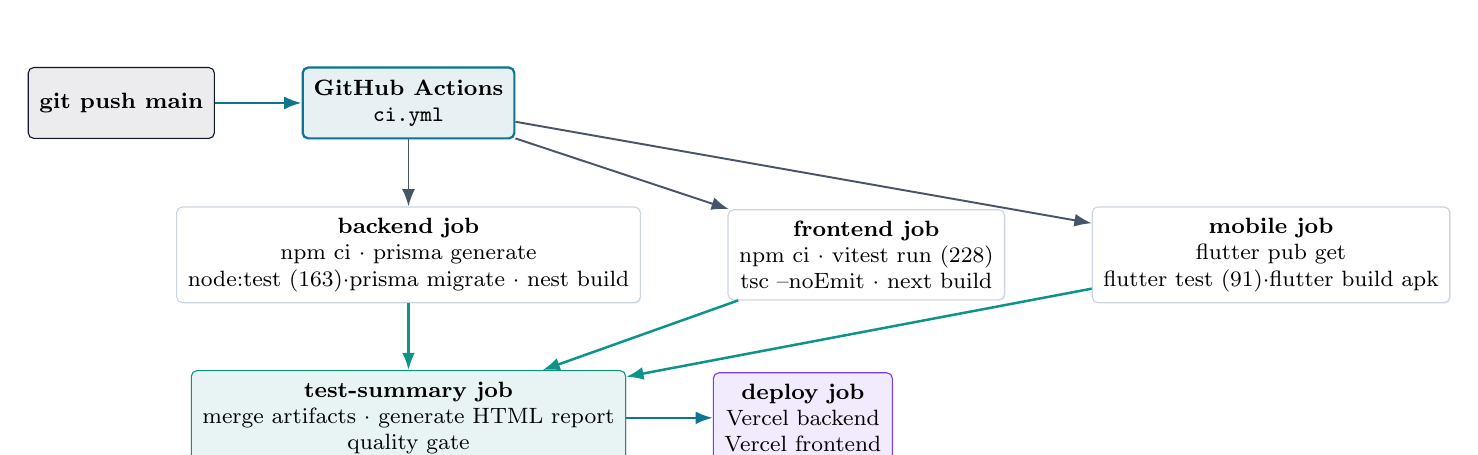
\begin{tikzpicture}[node distance=0.85cm and 1.1cm]
  \node[omniDarkNode] (push) {\textbf{git push main}};
  \node[omniAccent, right=of push] (gha) {\textbf{GitHub Actions}\\\texttt{ci.yml}};

  \node[omniNode, below=of gha] (be) {\bi{\textbf{backend job}}{\textbf{backend job}}\\npm ci $\cdot$ prisma generate\\node:test (163)$\cdot$prisma migrate $\cdot$ nest build};
  \node[omniNode, right=of be] (fe) {\bi{\textbf{frontend job}}{\textbf{frontend job}}\\npm ci $\cdot$ vitest run (228)\\tsc --noEmit $\cdot$ next build};
  \node[omniNode, right=of fe] (mob) {\bi{\textbf{mobile job}}{\textbf{mobile job}}\\flutter pub get\\flutter test (91)$\cdot$flutter build apk};

  \node[omniTealNode, below=of be] (sum) {\bi{\textbf{test-summary job}}{\textbf{test-summary job}}\\merge artifacts $\cdot$ generate HTML report\\quality gate};
  \node[omniPurpleNode, right=of sum] (dep) {\bi{\textbf{deploy job}}{\textbf{deploy job}}\\Vercel backend\\Vercel frontend};

  \draw[omniFlowAccent] (push) -- (gha);
  \draw[omniFlow] (gha) -- (be);
  \draw[omniFlow] (gha) -- (fe);
  \draw[omniFlow] (gha) -- (mob);
  \draw[omniFlowTeal] (be) -- (sum);
  \draw[omniFlowTeal] (fe) -- (sum);
  \draw[omniFlowTeal] (mob) -- (sum);
  \draw[omniFlowAccent] (sum) -- (dep);
\end{tikzpicture}%
}

% ------------------------------------------------------------
% Figure: JWT authentication & RBAC flow
% ------------------------------------------------------------
\newcommand{\figAuthFlow}{%
\begin{tikzpicture}[node distance=0.9cm and 1.2cm]
  \node[omniNode] (client) {\bi{\textbf{Client}}{\textbf{Client}}\\\bi{Web hoặc Mobile}{Web or Mobile}};
  \node[omniAccent, right=of client] (auth) {\textbf{AuthController}\\\texttt{/api/v1/auth/login}};
  \node[omniTealNode, right=of auth] (svc) {\textbf{AuthService}\\bcrypt verify\\deactivated check};
  \node[omniDarkNode, right=of svc] (db) {\textbf{PostgreSQL}\\\texttt{User} + \texttt{RefreshToken}};

  \node[omniPurpleNode, below=of svc] (tok) {\bi{\textbf{Cấp token}}{\textbf{Issue tokens}}\\\texttt{access} 60 min\\\texttt{refresh} 90 days (rotated)};
  \node[omniAmberNode, right=of tok] (guard) {\bi{\textbf{RBAC Guards}}{\textbf{RBAC Guards}}\\\texttt{JwtAuthGuard}\\\texttt{RolesGuard}};
  \node[omniRoseNode, right=of guard] (api) {\bi{\textbf{Endpoint có kiểm tra quyền}}{\textbf{Role-guarded endpoint}}\\\texttt{@Roles(1,2,3)}};

  \draw[omniFlowAccent] (client) -- (auth);
  \draw[omniFlowAccent] (auth) -- (svc);
  \draw[omniFlow] (svc) -- (db);
  \draw[omniFlowTeal] (svc) -- (tok);
  \draw[omniFlowTeal] (tok) -- (guard);
  \draw[omniFlowRose] (guard) -- (api);
  \draw[omniFlow, dashed] (client) to[out=0,in=180] node[above, font=\scriptsize] {Bearer token} (guard);
\end{tikzpicture}%
}

% ------------------------------------------------------------
% Figure: Ingest pipeline (external sources -> normalised events)
% ------------------------------------------------------------
\newcommand{\figIngest}{%
\begin{tikzpicture}[node distance=0.85cm and 1.2cm]
  \node[omniAmberNode] (yt) {\textbf{YouTube}\\Data API v3};
  \node[omniAmberNode, below=of yt] (tw) {\textbf{Twitch}\\Helix API};
  \node[omniAmberNode, below=of tw] (rss) {\textbf{RSS}\\Feed parser};

  \node[omniAccent, right=of yt] (cron) {\bi{\textbf{Bộ lập lịch}}{\textbf{Scheduler}}\\\texttt{@Cron}\\\bi{15'/30' phút}{15'/30' minutes}};
  \node[omniTealNode, right=of cron] (norm) {\bi{\textbf{Chuẩn hoá}}{\textbf{Normalise}}\\\texttt{NormalizedLiveEvent}\\duration in seconds};
  \node[omniDarkNode, right=of norm] (db) {\textbf{LiveEvent}\\\bi{upsert theo kênh}{upsert per channel}};
  \node[omniRoseNode, right=of db] (fill) {\bi{\textbf{Điền lịch trống}}{\textbf{EPG filler}}\\24/7 grid};

  \draw[omniFlowAmber] (yt) -- (cron);
  \draw[omniFlowAmber] (tw) -- (cron);
  \draw[omniFlowAmber] (rss) -- (cron);
  \draw[omniFlowAccent] (cron) -- (norm);
  \draw[omniFlowTeal] (norm) -- (db);
  \draw[omniFlowRose] (db) -- (fill);
\end{tikzpicture}%
}

% ------------------------------------------------------------
% Figure: End-to-End LiveStream & Live Studio Real-Time Architecture
% ------------------------------------------------------------
\newcommand{\figLiveStreamArch}{%
\begin{tikzpicture}[node distance=0.75cm and 1.1cm]
  % --- Broadcaster / Studio Sources (Left) ---
  \node[omniPurpleNode, minimum width=3.4cm] (tab1) at (0, 3.3) {\bi{\textbf{Tab 1: Chọn nội dung}}{\textbf{Tab 1: Curated Live}}\\VOD Library $\cdot$ Anti-piracy guard};
  \node[omniPurpleNode, minimum width=3.4cm] (tab2) at (0, 1.9) {\bi{\textbf{Tab 2: Tự ghi hình / Camera}}{\textbf{Tab 2: Self-Record / Camera}}\\WHIP WebRTC $\cdot$ Screen $\cdot$ Dropzone};
  \node[omniPurpleNode, minimum width=3.4cm] (tab3) at (0, 0.5) {\bi{\textbf{Tab 3: Kho công khai}}{\textbf{Tab 3: Public Catalog}}\\Verified HLS/MP4 $\cdot$ HEAD probe};
  \node[omniPurpleNode, minimum width=3.4cm] (tab4) at (0,-0.9) {\bi{\textbf{Tab 4: Điều hành \& Tương tác}}{\textbf{Tab 4: Host Control Console}}\\Pinned announcement $\cdot$ Stop/Switch};

  % --- Ingestion & Orchestration (Middle-Left) ---
  \node[omniAccent, minimum width=3.8cm, minimum height=1.5cm] (studio) at (4.6, 2.2) {\textbf{LiveStudioService}\\atomic event lifecycle\\\texttt{switchProgramOnLiveEvent}};
  \node[omniDarkNode, minimum width=3.8cm] (mtx) at (4.6, 0.5) {\textbf{MediaMTX + Cloudinary}\\WHIP/RTSP $\rightarrow$ WHEP/HLS (\texttt{.m3u8})\\Direct Drive proxy $\cdot$ Signed upload};
  \node[omniTealNode, minimum width=3.8cm, minimum height=1.5cm] (ws) at (4.6,-1.1) {\textbf{LiveStreamGateway (\texttt{/live})}\\Socket.IO rooms (\texttt{event:id})\\WebRTC SDP/ICE signalling};

  % --- Real-Time Events & Viewer Rooms (Right) ---
  \node[omniAmberNode, minimum width=4.0cm] (webroom) at (9.6, 2.5) {\bi{\textbf{Phòng Live Web (\texttt{/live/[id]})}}{\textbf{Web Live Room (\texttt{/live/[id]})}}\\7 genre lounges $\cdot$ Cinema mode\\Lineup switcher $\cdot$ Join Lobby};
  \node[omniAmberNode, minimum width=4.0cm] (mobroom) at (9.6, 0.7) {\bi{\textbf{Màn hình Mobile (\texttt{LiveWatch})}}{\textbf{Mobile \texttt{LiveWatchScreen}}}\\OmniPlayer $\cdot$ LAN host discovery\\Zero-cartoon exponential retry};
  \node[omniRoseNode, minimum width=4.0cm] (ops) at (9.6,-1.1) {\bi{\textbf{Thao tác Tương tác Tức thời}}{\textbf{Interactive Live Operations}}\\Chat \& Reply $\cdot$ 0ms Haptic Reactions\\6-Tier Super Chat $\cdot$ Host Toast};

  % --- Flows ---
  \draw[omniFlowAccent] (tab1) -- (studio);
  \draw[omniFlowAccent] (tab2) -- (studio);
  \draw[omniFlow] (tab2) -- (mtx);
  \draw[omniFlowAccent] (tab3) -- (studio);
  \draw[omniFlowTeal] (tab4) -- (ws);
  \draw[omniFlowTeal] (studio) -- (ws);
  \draw[omniFlow] (studio) -- (mtx);
  \draw[omniFlowAccent] (mtx) -- (webroom);
  \draw[omniFlowAccent] (mtx) -- (mobroom);
  \draw[omniFlowTeal] (ws) -- (webroom);
  \draw[omniFlowTeal] (ws) -- (mobroom);
  \draw[omniFlowRose] (ws) -- (ops);
  \draw[omniFlowRose, dashed] (ops) -- (mobroom);
  \draw[omniFlowRose, dashed] (ops) -- (webroom);
\end{tikzpicture}%
}

% ------------------------------------------------------------
% Figure: 5-Domain Relational Database Architecture (21 Prisma Models)
% ------------------------------------------------------------
\newcommand{\figDatabaseArchitecture}{%
\begin{tikzpicture}[node distance=0.8cm and 1.0cm]
  \node[omniAccent, minimum width=3.6cm, minimum height=2.1cm] (d1) at (0, 2.2) {\bi{\textbf{1. Định danh \& Bảo mật}}{\textbf{1. Identity \& Security}}\\\texttt{User} $\cdot$ \texttt{Role}\\\texttt{RefreshToken}};
  \node[omniTealNode, minimum width=4.0cm, minimum height=2.1cm] (d2) at (4.4, 2.2) {\bi{\textbf{2. Lõi Phát sóng \& EPG}}{\textbf{2. Broadcast Core \& EPG}}\\\texttt{Channel} $\cdot$ \texttt{Program}\\\texttt{Schedule} $\cdot$ \texttt{LiveEvent}\\\texttt{Category} $\cdot$ \texttt{ProgramCategory}};
  \node[omniPurpleNode, minimum width=4.0cm, minimum height=2.1cm] (d3) at (9.0, 2.2) {\bi{\textbf{3. Tương tác \& Thương mại}}{\textbf{3. Social \& Monetization}}\\\texttt{Comment} $\cdot$ \texttt{Reaction} $\cdot$ \texttt{Donation}\\\texttt{SubscriptionPlan} $\cdot$ \texttt{UserSubscription}\\\texttt{Watchlist} $\cdot$ \texttt{ViewHistory} $\cdot$ \texttt{FavoriteChannel}};
  \node[omniAmberNode, minimum width=4.2cm, minimum height=1.8cm] (d4) at (2.2,-0.5) {\bi{\textbf{4. Vận hành \& Kiểm toán gRPC}}{\textbf{4. Operations \& gRPC Audit}}\\\texttt{Notification} $\cdot$ \texttt{AuditLog}\\\texttt{WebhookSubscription}};
  \node[omniRoseNode, minimum width=4.2cm, minimum height=1.8cm] (d5) at (7.2,-0.5) {\bi{\textbf{5. Trí tuệ Nhân tạo (AI Curator)}}{\textbf{5. AI Content Intelligence}}\\\texttt{AiCuratorReport}\\\bi{1-1 với \texttt{Program} (sentiment/compliance)}{1-to-1 with \texttt{Program} (sentiment/compliance)}};

  \draw[omniFlowAccent] (d1) -- (d2);
  \draw[omniFlowTeal] (d2) -- (d3);
  \draw[omniFlow] (d1) -- (d3);
  \draw[omniFlowAmber] (d1) -- (d4);
  \draw[omniFlowRose] (d2) -- (d5);
\end{tikzpicture}%
}

% ------------------------------------------------------------
% Figure: Complete Mobile Navigation & 31-Screen Hierarchy (PRM393)
% ------------------------------------------------------------
\newcommand{\figMobileScreenMap}{%
\begin{tikzpicture}[node distance=0.65cm and 0.9cm]
  \node[omniDarkNode, minimum width=3.6cm] (root) at (4.5, 3.6) {\textbf{GoRouter Root}\\Splash $\cdot$ Onboarding $\cdot$ Auth (4)};

  \node[omniAccent, minimum width=3.8cm] (shell) at (4.5, 2.1) {\textbf{MainNavigationShell (6 Tabs)}\\Home $\cdot$ Channels $\cdot$ Schedule\\Saved $\cdot$ History $\cdot$ Profile};

  \node[omniRoseNode, minimum width=3.5cm] (live) at (0.2, 0.4) {\bi{\textbf{Cụm Xem Live \& VOD}}{\textbf{Live \& VOD Cluster}}\\\texttt{LiveNowScreen} (\texttt{/live})\\\texttt{LiveWatchScreen} (\texttt{/live/:id})\\\texttt{OmniPlayer} + Super Chat + Chat};

  \node[omniPurpleNode, minimum width=3.6cm] (studio) at (4.5, 0.4) {\bi{\textbf{Cụm Studio Phát sóng}}{\textbf{Broadcast Studio Cluster}}\\\texttt{LiveStudioScreen} (4 Tabs)\\\texttt{MobileStudioRecorderScreen}\\Teleprompter $\cdot$ VU Meter $\cdot$ QC};

  \node[omniTealNode, minimum width=3.5cm] (admin) at (8.8, 0.4) {\bi{\textbf{Cụm Quản trị \& AI}}{\textbf{Admin \& AI Cluster}}\\\texttt{AdminManageScreen} (4 Tabs)\\\texttt{AiCuratorScreen} $\cdot$ Schedule Form\\Notifications $\cdot$ Settings $\cdot$ Sub Plans};

  \draw[omniFlowAccent] (root) -- (shell);
  \draw[omniFlowRose] (shell) -- (live);
  \draw[omniFlow] (shell) -- (studio);
  \draw[omniFlowTeal] (shell) -- (admin);
\end{tikzpicture}%
}


\begin{document}

% ============================================================
% PRM393 - Academic Cover Page (Trang Bìa Đồ Án FPT University)
% ============================================================
\onecolumn
\thispagestyle{empty}

\begin{tikzpicture}[remember picture, overlay]
  % Khung viền đôi trang trọng
  \draw[line width=2pt, color=omniDark] 
    ($(current page.north west) + (20mm,-20mm)$) 
    rectangle 
    ($(current page.south east) + (-15mm,20mm)$);
  \draw[line width=0.8pt, color=omniBlue] 
    ($(current page.north west) + (21.5mm,-21.5mm)$) 
    rectangle 
    ($(current page.south east) + (-16.5mm,21.5mm)$);
  \fill[omniBlue] ($(current page.north west) + (21.5mm,-21.5mm)$) circle (2.5pt);
  \fill[omniBlue] ($(current page.north east) + (-16.5mm,-21.5mm)$) circle (2.5pt);
  \fill[omniBlue] ($(current page.south west) + (21.5mm,21.5mm)$) circle (2.5pt);
  \fill[omniBlue] ($(current page.south east) + (-16.5mm,21.5mm)$) circle (2.5pt);
\end{tikzpicture}

\begin{center}
  \vspace*{-7mm}
  {\bfseries\large\bi{BỘ GIÁO DỤC VÀ ĐÀO TẠO}{MINISTRY OF EDUCATION AND TRAINING}}\\[1.5mm]
  {\bfseries\Large\bi{TRƯỜNG ĐẠI HỌC FPT --- FPTU QUY NHON AI CAMPUS}{FPT UNIVERSITY --- FPTU QUY NHON AI CAMPUS}}\\[1.5mm]
  {\small\bfseries\textcolor{omniBlue}{FU CAHATA $\cdot$ \bi{KHOA CÔNG NGHỆ THÔNG TIN --- BỘ MÔN KỸ THUẬT PHẦN MỀM}{FACULTY OF INFORMATION TECHNOLOGY --- SOFTWARE ENGINEERING}}}\\[5mm]

  % Huy hiệu nhận diện ứng dụng OmniCast Mobile
  \begin{tikzpicture}
    \node[draw=omniBlue, fill=omniLight, rounded corners=6pt, line width=1.2pt, inner sep=6pt] {
      \textbf{\large\textcolor{omniDark}{OMNI}\textcolor{omniBlue}{CAST MOBILE}}
      \quad\textcolor{omniSlate}{\footnotesize$\vert$}\quad
      \textcolor{omniDark}{\footnotesize\bfseries\bi{ỨNG DỤNG DI ĐỘNG NATIVE FLUTTER}{NATIVE FLUTTER CLIENT}}
    };
  \end{tikzpicture}
  \vspace{5mm}

  {\Large\bfseries\bi{BÁO CÁO NGHIỆM THU ĐỒ ÁN HỌC PHẦN}{FINAL PROJECT DELIVERABLE REPORT}}\\[2.5mm]
  {\large\bfseries\bi{HỌC PHẦN: PRM393 --- PHÁT TRIỂN ỨNG DỤNG DI ĐỘNG}{COURSE: PRM393 --- MOBILE APPLICATIONS DEVELOPMENT}}\\[5mm]

  {\color{omniBlue}\rule{0.85\linewidth}{1.6pt}}\\[4mm]
  {\LARGE\bfseries\bi{ỨNG DỤNG DI ĐỘNG PHÁT SÓNG VÀ}{OMNICAST MOBILE: ENTERPRISE BROADCAST}}\\[2mm]
  {\LARGE\bfseries\bi{TRUYỀN HÌNH TRỰC TUYẾN OMNICAST MOBILE}{\& INTERACTIVE STREAMING CLIENT}}\\[2.5mm]
  {\large\bfseries\textcolor{omniBlue}{Cross-Platform Broadcast \& Interactive Multimedia Streaming Client}}\\[2mm]
  {\normalsize\itshape\bi{Kiến trúc Clean Architecture 4 tầng, Quản lý trạng thái BLoC, Phòng xem LiveStream \& Bàn điều khiển Mobile Live Studio (WebRTC WHIP), Bộ nhớ đệm SQLite Offline-First và Trình phát OmniPlayer}{4-Tier Clean Architecture, BLoC State Management, Interactive LiveStream \& Mobile Live Studio (WebRTC WHIP), Offline-First SQLite Cache, and Ultra-Low Latency OmniPlayer}}\\[3.5mm]
  {\color{omniBlue}\rule{0.85\linewidth}{1.6pt}}\\[5mm]

  \begin{tcolorbox}[
    colback=white, colframe=omniBorder, boxrule=0.8pt, arc=3pt,
    width=0.90\linewidth, left=6mm, right=6mm, top=3.5mm, bottom=3.5mm
  ]
  \renewcommand{\arraystretch}{1.24}
  \footnotesize
  \begin{tabular}{p{4.3cm}p{8.8cm}}
    \textbf{\bi{Giảng viên hướng dẫn (Mentor):}{Mentor / Supervisor:}} & \textbf{\bi{Thầy Huỳnh Vang}{Mr. Huỳnh Vang}} (\bi{Bộ môn Kỹ thuật Phần mềm --- FPTU}{Software Engineering Dept. --- FPTU}) \\
    \textbf{\bi{Đơn vị \& Câu lạc bộ:}{Campus \& Team Note:}}          & \textbf{FPTU Quy Nhon AI Campus --- FU Cahata} \\
    \textbf{\bi{Học kỳ thực hiện:}{Academic Semester:}}                & Fall 2026 (FA26) \\
    \textbf{\bi{Thành viên nhóm (4 TV):}{Project Team Members (4):}}   & \textbf{1. Nguyễn Bình An} (\bi{Nhóm trưởng / Kiến trúc Backend \& Bảo mật}{Team Leader / Backend \& Security}) \\
                                                                       & \textbf{2. Trần Thanh Sơn} --- MSSV: \texttt{QE170080} (\bi{gRPC Audit \& Cơ sở dữ liệu}{gRPC Audit \& Database}) \\
                                                                       & \textbf{3. Nguyễn Vĩnh Phú} --- MSSV: \texttt{QE180136} (\bi{Trưởng nhóm Mobile Flutter}{Mobile Flutter Lead}) \\
                                                                       & \textbf{4. Đồng Hoàng Nguyên} (\bi{Full-Stack Next.js, LiveStream \& AI Curator}{Full-Stack Web, Live \& AI}) \\
    \textbf{\bi{Kho mã nguồn (GitHub):}{GitHub Repository:}}           & \url{https://github.com/TomOutfit/OmniCast_PRN232-PRM393_Project_Fa26Semester} \\
    \textbf{\bi{Bản phát hành APK:}{Mobile Release (APK):}}            & \url{https://github.com/TomOutfit/OmniCast_PRN232-PRM393_Project_Fa26Semester/releases/tag/v1.2.0} \\
    \textbf{\bi{Quy mô \& Kiểm định:}{Scale \& Verification:}}         & \textbf{\bi{53.922 dòng mã Dart $\vert$ 31 Màn hình $\vert$ 91/91 Tests PASS (100\%)}{53,922 Dart LOC $\vert$ 31 Screens $\vert$ 91/91 Tests PASS (100\%)}} \\
  \end{tabular}
  \end{tcolorbox}

  \vfill
  {\bfseries\bi{FPTU QUY NHON AI CAMPUS --- FU CAHATA $\cdot$ THÁNG 10 NĂM 2026}{FPTU QUY NHON AI CAMPUS --- FU CAHATA $\cdot$ OCTOBER 2026}}\\[2mm]
\end{center}

\clearpage
\twocolumn


\pagenumbering{arabic}
\setcounter{page}{1}
\pagestyle{fancy}

\title{\bi{Phát triển ứng dụng di động đa nền tảng: Ứng dụng phát thanh truyền hình và phân phối nội dung số OmniCast Mobile}{Cross-Platform Mobile Application Development: The OmniCast Mobile Broadcast and Digital Content Delivery Client}}

\author{\IEEEauthorblockN{\textbf{Nguyễn Bình An}, \textbf{Trần Thanh Sơn} (\texttt{QE170080}), \textbf{Nguyễn Vĩnh Phú} (\texttt{QE180136}), \textbf{Đồng Hoàng Nguyên}}\\
\IEEEauthorblockA{\bi{Giảng viên hướng dẫn (Mentor): \textbf{Thầy Huỳnh Vang}}{Mentor / Supervisor: \textbf{Mr. Huỳnh Vang}}\\
\textbf{FPTU Quy Nhon AI Campus --- FU Cahata}, \bi{Khoa Công nghệ Thông tin, Trường Đại học FPT}{Faculty of Information Technology, FPT University}\\
\bi{Kho mã nguồn}{Source Code}: \url{https://github.com/TomOutfit/OmniCast_PRN232-PRM393_Project_Fa26Semester} $\cdot$ \bi{Bản cài đặt APK}{Release APK}: \url{https://github.com/TomOutfit/OmniCast_PRN232-PRM393_Project_Fa26Semester/releases/tag/v1.2.0}}}
\date{}

\maketitle
\thispagestyle{fancy}

\begin{abstract}
\bi{
OmniCast Mobile là ứng dụng di động phân phối nội dung số và phát thanh truyền
hình trực tiếp (LiveStream) đa nền tảng được xây dựng tại FPTU Quy Nhon AI Campus --- FU Cahata cho môn học PRM393 dưới sự hướng dẫn của thầy Huỳnh Vang bằng Flutter 3.x
và ngôn ngữ Dart. Ứng dụng tích hợp kiến trúc phân tầng Clean Architecture 4 lớp kết
hợp mô hình quản lý trạng thái luồng phản ứng BLoC với 12 module nghiệp vụ và 31 màn hình chuyên biệt. Bốn
đóng góp kỹ thuật trọng tâm bao gồm: (1) trình
phát đa năng \texttt{OmniPlayer} tích hợp luồng phát trực tiếp độ trễ thấp WebRTC/HLS
từ MediaMTX, phân giải luồng trực tiếp Google Drive, tự động khám phá máy chủ nội bộ qua Wi-Fi (\texttt{LanDiscoveryService})
và phòng xem tương tác thời gian thực hai chiều (\texttt{LiveWatchScreen}: Live Chat phân nhánh, biểu cảm hạt nổi xúc giác 0ms, quyên góp Super Chat 6 mệnh giá, thông báo ghim từ Host và chuyển chương trình tức thời); (2) bàn điều khiển \texttt{LiveStudioScreen} 4 tab cùng máy quay tác nghiệp hiện trường \texttt{MobileStudioRecorderScreen} hỗ trợ đẩy sóng WebRTC WHIP trực tiếp, mã thời gian SMPTE, đồng hồ âm lượng Stereo VU Meter và máy nhắc chữ Teleprompter HUD; (3) động cơ ngoại tuyến (offline-first) trên
nền cơ sở dữ liệu SQLite cục bộ với hàng đợi phát lại thao tác bất đồng bộ
(\texttt{pending\_ops}) và thông báo nhắc lịch chính xác trước 15 phút; cùng (4) hệ thống điều hướng tập trung GoRouter quản lý 31 màn
hình với cơ chế bảo vệ phiên đăng nhập chặt chẽ. Hệ thống đã được kiểm chứng
thông qua 91 ca kiểm thử tự động đạt tỷ lệ vượt qua 100\% trong quy trình CI/CD
GitHub Actions.
}{
OmniCast Mobile is an enterprise cross-platform digital broadcast, LiveStream and
multimedia streaming client engineered at FPTU Quy Nhon AI Campus --- FU Cahata for the PRM393 course under the supervision of Mentor Mr. Huỳnh Vang utilizing
Flutter 3.x and Dart. The client adheres to a 4-tier Clean Architecture
coupled with reactive stream-based BLoC state management spanning 12 business
modules and 31 screens. Four core technological contributions are presented: (1) the multi-engine
\texttt{OmniPlayer} uniting ultra-low-latency WebRTC/HLS streams via MediaMTX, direct Google Drive stream resolution, dynamic Wi-Fi
LAN host discovery (\texttt{LanDiscoveryService}), and bi-directional real-time interactive live rooms (\texttt{LiveWatchScreen}: threaded Live
Chat, 0ms haptic Floating Reactions, 6-tier Super Chat Donations, pinned broadcaster banners and zero-downtime program switching); (2) a 4-tab \texttt{LiveStudioScreen} and professional field-reporter camera viewfinder (\texttt{MobileStudioRecorderScreen}) featuring Push-to-Live WebRTC WHIP publishing, SMPTE timecode, Stereo VU audio meters and an auto-scrolling Teleprompter HUD; (3) an
offline-first engine driven by local SQLite storage featuring an asynchronous
mutation replay queue (\texttt{pending\_ops}) and exact 15-minute advance local alarms; and (4) a declarative GoRouter topology
governing 31 screens with strict session-guarded route protection. The software
architecture is verified by 91 automated unit and widget tests achieving a
100\% pass rate on GitHub Actions CI runners.
}
\end{abstract}

\begin{IEEEkeywords}
\bi{Flutter, Dart, BLoC, LiveStream, Live Studio, WebRTC WHIP, SQLite, offline-first, MediaMTX, HLS, GoRouter, FPTU Quy Nhon AI Campus, FU Cahata.}{Flutter, Dart, BLoC, LiveStream, Live Studio, WebRTC WHIP, SQLite, offline-first, MediaMTX, HLS, GoRouter, FPTU Quy Nhon AI Campus, FU Cahata.}
\end{IEEEkeywords}

% ============================================================
% PRM393 - Section 1: Introduction (Bilingual)
% ============================================================
\section{\bi{Mở đầu}{Introduction}}
\label{sec:intro}

\bi{
Trong kỷ nguyên phân phối nội dung số hiện đại, ứng dụng di động đã trở
thành điểm tiếp xúc chính yếu giữa người dùng và các dịch vụ truyền thông
trực tuyến. Khác với môi trường máy tính để bàn (web desktop) có đường
truyền mạng ổn định và nguồn năng lượng dồi dào, môi trường di động đặt ra
những thách thức kỹ thuật nghiêm ngặt: độ trễ mạng biến động liên tục, kết
nối thường xuyên bị gián đoạn khi chuyển vùng (cell tower handover / Wi-Fi
to cellular), hạn chế về bộ nhớ RAM và thời lượng pin thiết bị.

Để giải quyết toàn diện các thách thức trên, bài báo này trình bày thiết
kế và hiện thực ứng dụng di động \textbf{OmniCast Mobile} --- một ứng dụng
phát thanh truyền hình, truyền phát trực tiếp (LiveStream) và phân phối nội dung số đa nền tảng được nghiên cứu và phát triển tại \textbf{FPTU Quy Nhon AI Campus --- FU Cahata}
cho môn học \textbf{PRM393 --- Mobile Applications Development} dưới sự hướng dẫn chuyên môn của giảng viên (\emph{Mentor}) \textbf{Thầy Huỳnh Vang}. Ứng dụng
được xây dựng trên nền tảng Flutter 3.x với ngôn ngữ Dart (53.922 dòng mã Dart), áp dụng kiến trúc
phân tầng Clean Architecture 4 lớp kết hợp mô hình quản lý trạng thái BLoC (Business Logic
Component) điều phối 31 màn hình và 22 thành phần giao diện chuyên dụng.
}{
In the modern era of digital content delivery, mobile applications have
become the primary touchpoint connecting viewers with broadcast media
services. Unlike desktop environments with steady broadband connectivity
and continuous power supplies, mobile devices present stringent technical
challenges: highly fluctuating network latency, frequent network drops during
roaming transitions (cell tower handovers or Wi-Fi to cellular switches),
constrained memory footprints, and battery budget limits.

To comprehensively address these demands, this paper presents the
architectural design and implementation of \textbf{OmniCast Mobile} --- an
enterprise cross-platform digital broadcast, LiveStream and multimedia streaming client
developed at \textbf{FPTU Quy Nhon AI Campus --- FU Cahata} for the course \textbf{PRM393 --- Mobile Applications Development} under the academic mentorship of \textbf{Mr. Huỳnh Vang}.
Built upon Flutter 3.x with the Dart language (53,922 Dart LOC), the client adopts a clean
four-tier layered architecture coupled with the Business Logic Component
(BLoC) state management pattern across 31 screens and 22 custom widgets.
}

\subsection{\bi{Động lực và bài toán kỹ thuật}{Motivation and Engineering Challenges}}

\bi{
Quá trình xây dựng ứng dụng di động OmniCast tập trung vào việc giải quyết năm
bài toán kỹ thuật cốt lõi:
}{
The engineering of OmniCast Mobile resolves five pivotal technical
challenges:
}

\begin{enumerate}[leftmargin=*,itemsep=2pt]
  \item \bi{\textbf{Khả năng hoạt động khi mất mạng (Offline-First):}
  Người dùng thường xuyên tra cứu lịch phát sóng (EPG) và danh sách theo
  dõi (Watchlist) trong điều kiện mất kết nối. Ứng dụng phải hỗ trợ lưu
  trữ cục bộ bằng cơ sở dữ liệu SQLite, xếp hàng các thao tác phát sinh khi
  ngoại tuyến và tự động phát lại (replay) đồng bộ lên máy chủ khi có mạng
  trở lại.}{%
  \textbf{Offline-First Resilience:} Viewers frequently consult electronic
  programme guides (EPG) and their personal watchlists in poor or nonexistent
  connectivity conditions. The application must store structured data in a
  local SQLite database, queue pending mutations while offline, and seamlessly
  replay them to the central cloud upon reconnection.}

  \item \bi{\textbf{Luồng phát đa phương tiện độ trễ thấp và tự động khám phá mạng LAN:}
  Hệ sinh thái OmniCast phát sóng qua nhiều giao thức: WebRTC / HLS thông
  qua MediaMTX, luồng trực tiếp Google Drive và luồng nhúng video ngoài. Trình phát \texttt{OmniPlayer}
  phải tự động quét và khám phá địa chỉ IP máy chủ MediaMTX trong mạng Wi-Fi cục bộ (\texttt{LanDiscoveryService}) và tự phục hồi
  khi luồng video bị đứt quãng.}{%
  \textbf{Low-Latency Adaptive Streaming and LAN Host Discovery:} The OmniCast broadcast pipeline
  emits ultra-low-latency WebRTC/HLS streams via MediaMTX, direct Google Drive streams, and external
  curated feeds. The embedded \texttt{OmniPlayer} must dynamically scan and discover
  local Wi-Fi MediaMTX hosts (\texttt{LanDiscoveryService}) and recover transparently during transient
  network drops.}

  \item \bi{\textbf{Phòng xem LiveStream tương tác hai chiều \& Bàn điều khiển Mobile Live Studio:}
  Người xem không chỉ thụ động tiếp nhận luồng phát mà còn tham gia sảnh chờ, gửi bình luận phân nhánh,
  thả biểu cảm hạt nổi có phản hồi xúc giác 0ms, nhận thông báo ghim từ đạo diễn và quyên góp Super Chat 6 mệnh giá. Đồng thời, phóng viên hiện trường cần một bàn điều khiển \texttt{LiveStudioScreen} 4 tab và ống kính máy quay \texttt{MobileStudioRecorderScreen} hỗ trợ đẩy sóng WebRTC WHIP trực tiếp từ điện thoại.}{%
  \textbf{Bi-Directional Interactive LiveStream \& Mobile Live Studio:} Viewers expect rich interactive
  rooms with lobby prompts, threaded live chat, 0ms haptic floating reactions, pinned host banners, and 6-tier Super Chat donations. Meanwhile, field reporters require a 4-tab \texttt{LiveStudioScreen} and hardware camera viewfinder (\texttt{MobileStudioRecorderScreen}) capable of real-time WebRTC WHIP publishing.}

  \item \bi{\textbf{Quản lý trạng thái phân tán và bảo mật phiên:}
  Việc điều hướng 31 màn hình với 12 module BLoC yêu cầu cơ chế kiểm soát
  trạng thái chặt chẽ, cùng với việc lưu trữ token JWT an toàn trong
  Keystore/Keychain để tự động gia hạn phiên làm việc ngầm mà không làm phiền
  người dùng.}{%
  \textbf{Distributed State Management and Session Security:}
  Navigating 31 screens powered by 12 BLoC modules requires predictable
  unidirectional data flows, paired with hardware-backed secure storage
  (Keystore/Keychain) for transparent JWT token rotation.}
\end{enumerate}

\subsection{\bi{Tổ chức nhóm nghiên cứu và Phân công nhiệm vụ}{Project Team Organization and Role Allocation}}

\bi{
Dự án được thực hiện bởi nhóm 4 sinh viên tại \textbf{FPTU Quy Nhon AI Campus --- FU Cahata} dưới sự hướng dẫn của giảng viên \textbf{Thầy Huỳnh Vang}, như trình bày tại Bảng~\ref{tab:team_prm}.
}{
The project was executed by a four-member student engineering team at \textbf{FPTU Quy Nhon AI Campus --- FU Cahata} under the supervision of Mentor \textbf{Mr. Huỳnh Vang}, as detailed in Table~\ref{tab:team_prm}.
}

\begin{table}[t]
\caption{\bi{Danh sách 4 thành viên nhóm dự án OmniCast (FPTU Quy Nhon AI Campus --- FU Cahata, Mentor: Thầy Huỳnh Vang).}{The 4 project team members of OmniCast (FPTU Quy Nhon AI Campus --- FU Cahata, Mentor: Mr. Huỳnh Vang).}}
\label{tab:team_prm}
\centering
\scriptsize
\begin{tabular}{@{}p{2.3cm}p{1.5cm}p{4.3cm}@{}}
\toprule
\textbf{\bi{Họ và tên}{Full Name}} & \textbf{\bi{Vai trò / MSSV}{Role / ID}} & \textbf{\bi{Phụ trách kỹ thuật chính}{Primary Engineering Ownership}} \\
\midrule
\textbf{Nguyễn Bình An} (\texttt{TomOutfit}) & \bi{Nhóm trưởng}{Team Leader} & \bi{Kiến trúc lõi NestJS 19 module, Bảo mật JWT \& RBAC 4 vai trò, Thuật toán chống xung đột lịch EPG, Direct Stream Engine, CI/CD \& Triển khai}{NestJS 19-module core architecture, JWT \& 4-role RBAC security, EPG conflict detection SQL, Direct Stream Engine, CI/CD \& Release} \\
\addlinespace[2pt]
\textbf{Trần Thanh Sơn} & \texttt{QE170080} & \bi{Kiến trúc vi dịch vụ gRPC Audit Logger (\texttt{audit\_logger.proto}), Cơ sở dữ liệu PostgreSQL Supabase (21 Prisma models), Telemetry \& Seed}{Standalone gRPC Audit Logger microservice (\texttt{audit\_logger.proto}), Supabase PostgreSQL (21 Prisma models), Telemetry \& Seeding} \\
\addlinespace[2pt]
\textbf{Nguyễn Vĩnh Phú} & \texttt{QE180136} & \bi{Trưởng nhóm Mobile Flutter (31 màn hình, 12 BLoC), Trình phát \texttt{OmniPlayer}, \texttt{MobileStudioRecorderScreen} (WebRTC WHIP), Offline SQLite}{Mobile Flutter Lead (31 screens, 12 BLoCs), \texttt{OmniPlayer} engine, \texttt{MobileStudioRecorderScreen} (WebRTC WHIP), Offline SQLite} \\
\addlinespace[2pt]
\textbf{Đồng Hoàng Nguyên} (\texttt{teng122}) & Full-Stack \& AI & \bi{Cổng Web Next.js 15 Cinema Dark (33 route), Cổng Socket.IO \texttt{/live}, Phòng Live 7 chủ đề, Bàn điều khiển Live Studio \& Module AI Curator}{Next.js 15 Cinema Dark Web Portal (33 routes), Socket.IO \texttt{/live} gateway, 7-theme Live Room, Live Studio Console \& AI Curator module} \\
\bottomrule
\end{tabular}
\end{table}

\subsection{\bi{Đóng góp chính của báo cáo}{Principal Contributions}}

\bi{
Báo cáo này phân tích chi tiết năm đóng góp công nghệ của ứng dụng:
}{
This paper details five principal technical contributions:
}

\begin{itemize}[leftmargin=*,itemsep=2pt]
  \item \bi{Kiến trúc Clean Architecture 4 tầng (Presentation, Logic/BLoC,
  Data, Core) với cơ chế Service Locator qua \texttt{get\_it}.}{%
  A 4-tier Clean Architecture (Presentation, Logic/BLoC, Data, Core)
  orchestrated through \texttt{get\_it} service locator.}
  \item \bi{Hệ sinh thái \texttt{OmniPlayer}, \texttt{LiveWatchScreen}, \texttt{LiveStudioScreen} (4 tab) và máy quay \texttt{MobileStudioRecorderScreen} (WebRTC WHIP, SMPTE Timecode, Stereo VU Meter, Teleprompter HUD).}{%
  A complete mobile live broadcast ecosystem comprising \texttt{OmniPlayer}, \texttt{LiveWatchScreen}, the 4-tab \texttt{LiveStudioScreen} and the \texttt{MobileStudioRecorderScreen} field viewfinder (WebRTC WHIP, SMPTE timecode, Stereo VU meter, Teleprompter HUD).}
  \item \bi{Mô hình quản lý trạng thái luồng (Stream-based BLoC) với các
  concurrency transformer như \texttt{droppable} và \texttt{restartable}.}{%
  A stream-based reactive state architecture employing custom BLoC
  concurrency transformers such as \texttt{droppable} and \texttt{restartable}.}
  \item \bi{Động cơ ngoại tuyến SQLite với hàng đợi \texttt{pending\_ops} và cơ chế tự
  động giải quyết xung đột dữ liệu.}{%
  An offline-first SQLite synchronization engine featuring an asynchronous
  mutation queue (\texttt{pending\_ops}) and conflict resolution heuristics.}
  \item \bi{Bộ kiểm thử tự động toàn diện gồm 91 test đạt tỷ lệ vượt qua
  100\% trên quy trình CI/CD GitHub Actions.}{%
  A test suite of 91 automated unit and widget tests achieving a 100\%
  pass rate in a GitHub Actions continuous integration matrix.}
\end{itemize}

% ============================================================
% PRM393 - Section 2: Architecture & Foundation (Bilingual)
% ============================================================
\section{\bi{Kiến trúc ứng dụng di động}{Mobile System Architecture}}
\label{sec:arch}

\bi{
OmniCast Mobile tuân thủ triệt để nguyên lý phân tách trách nhiệm (Separation
of Concerns) và kiến trúc Clean Architecture được điều chỉnh cho hệ sinh thái
Flutter. Cấu trúc mã nguồn được phân chia thành bốn tầng độc lập:
Presentation, Logic (BLoC), Data và Core, bảo đảm tính độc lập khi kiểm thử
(testability), khả năng tái sử dụng mã nguồn và tính dễ bảo trì.
}{
OmniCast Mobile strictly adheres to the Separation of Concerns and Clean
Architecture principles adapted for the Flutter framework. The codebase is
organized into four distinct layers: Presentation, Logic (BLoC), Data, and
Core, ensuring high testability, modular reusability, and long-term
maintainability.
}

\begin{figure}[t]
\centering
\fitcol{\figMobileArchitecture}
\caption{\bi{Sơ đồ kiến trúc phân tầng 4 lớp của ứng dụng di động OmniCast:
tầng Presentation điều hướng qua GoRouter (31 màn hình, 22 widget), tầng Logic với 12 BLoC/Cubit, tầng
Data giao tiếp đồng thời với REST API, Socket.IO \texttt{/live} và SQLite ngoại tuyến.}{The 4-tier
layered architecture of OmniCast Mobile: Presentation routed by GoRouter (31 screens, 22 widgets),
Logic driven by 12 BLoC/Cubits, and Data communicating concurrently with
NestJS REST APIs, Socket.IO \texttt{/live} and local SQLite storage.}}
\label{fig:mob_arch}
\end{figure}

\begin{figure*}[t]
\centering
\fitfull{\figLiveStreamArch}
\caption{\bi{Kiến trúc truyền phát trực tiếp (LiveStream) và bàn điều khiển Live Studio đầu-cuối giữa ứng dụng di động Flutter, cổng Web Next.js 15, máy chủ MediaMTX (WHIP/WHEP/HLS) và cổng Socket.IO \texttt{/live}.}{End-to-end LiveStream and Live Studio architecture bridging the Flutter mobile client, Next.js 15 web portal, MediaMTX (WHIP/WHEP/HLS) and the Socket.IO \texttt{/live} gateway.}}
\label{fig:mob_livestream_arch}
\end{figure*}

\subsection{\bi{Phân tầng trách nhiệm}{Layered Organization}}

\bi{
Bốn tầng kiến trúc được tổ chức như sau:
}{
The four architectural tiers are defined as follows:
}

\begin{enumerate}[leftmargin=*,itemsep=2pt]
  \item \textbf{Presentation Layer:} \bi{Gồm 31 màn hình (screens) và 22
  thành phần giao diện tái sử dụng (widgets). Tầng này hoàn toàn không chứa
  logic nghiệp vụ phức tạp mà chỉ chịu trách nhiệm hiển thị trạng thái và
  phát sinh các sự kiện người dùng (User Events).}{%
  Encompasses 31 screens and 22 reusable widgets. This tier is completely free
  of business computations, focusing solely on state rendering and event
  dispatching.}

  \item \textbf{Logic Layer (BLoC / Cubit):} \bi{Gồm 12 module điều phối
  nghiệp vụ. BLoC tiếp nhận sự kiện từ Presentation, giao tiếp với tầng Data
  qua các Repository và phát ra các trạng thái mới (States) thông qua các
  Stream bất đồng bộ.}{%
  Hosts 12 state-management modules. BLoCs accept incoming events from UI
  widgets, invoke domain repositories, and emit reactive state streams.}

  \item \textbf{Data Layer:} \bi{Chứa 10 Repository, Data Sources và 10 Model
  dữ liệu. Tầng này trừu tượng hóa nguồn gốc dữ liệu: tự động quyết định đọc
  từ bộ nhớ đệm SQLite hay gọi mạng từ xa qua Dio Client.}{%
  Encapsulates 10 Repositories, Data Sources, and 10 Data Transfer Objects (DTOs).
  It abstracts data origins, transparently querying SQLite or fetching
  remotely via Dio.}

  \item \textbf{Core Layer:} \bi{Cung cấp các tiện ích dùng chung: bộ định
  tuyến \texttt{GoRouter}, bộ tiêm phụ thuộc \texttt{get\_it}, dịch vụ khám phá máy chủ phát sóng nội bộ \texttt{LanDiscoveryService}, dịch vụ đẩy luồng \texttt{WebRTCPublisherService}, cấu hình
  giao diện (theme), chuỗi bản địa hóa (i18n), dịch vụ thông báo cục bộ và
  quản lý token bảo mật.}{%
  Supplies cross-cutting concerns: \texttt{GoRouter} navigation definitions,
  \texttt{get\_it} dependency injection, \texttt{LanDiscoveryService} Wi-Fi subnet scanner, \texttt{WebRTCPublisherService} WHIP streamer, UI theme styling, i18n
  localization, and secure token storage.}
\end{enumerate}

\subsection{\bi{Bộ tiêm phụ thuộc (Dependency Injection)}{Dependency Injection with GetIt}}

\bi{
Toàn bộ các thực thể Repository, Data Source, HTTP Client và BLoC được khởi
tạo và quản lý vòng đời thông qua thư viện \texttt{get\_it}. Trong tệp
\texttt{injection\_container.dart}, cơ chế đăng ký được phân định rõ ràng
giữa Lazy Singleton (cho các dịch vụ mạng, cơ sở dữ liệu và repository) và
Factory (cho các BLoC cần tạo mới theo vòng đời màn hình):
}{
All Repositories, Data Sources, Network Clients, and BLoC instances have
their lifecycles managed via the \texttt{get\_it} service locator. In
\texttt{injection\_container.dart}, registrations are strictly partitioned
between Lazy Singletons (for stateless services, DB helpers, and repositories)
and Factories (for transient BLoC instances tied to screen lifecycles):
}

\begin{lstlisting}[language=Dart, caption={\bi{Cấu hình tiêm phụ thuộc trong \texttt{injection\_container.dart}.}{Dependency injection configuration in \texttt{injection\_container.dart}.}}]
final sl = GetIt.instance;

Future<void> init() async {
  // BLoCs (Factory)
  sl.registerFactory(() => AuthBloc(sl()));
  sl.registerFactory(() => WatchlistBloc(sl()));
  sl.registerFactory(() => EpgBloc(sl()));

  // Repositories (Lazy Singleton)
  sl.registerLazySingleton<WatchlistRepository>(
    () => WatchlistRepositoryImpl(
      remoteDataSource: sl(),
      localDataSource: sl(),
    ),
  );

  // Core & Drivers
  sl.registerLazySingleton(() => DioClient(sl()));
  sl.registerLazySingleton(() => DatabaseHelper());
}
\end{lstlisting}

\subsection{\bi{Tầng mạng và xoay vòng Token bảo mật}{Networking and JWT Token Rotation}}

\bi{
Giao tiếp HTTP được thực hiện qua thư viện \texttt{Dio} với lớp đánh chặn
\texttt{AuthInterceptor}. Khi ứng dụng nhận mã lỗi \texttt{HTTP 401
Unauthorized}, bộ đánh chặn sẽ tự động kích hoạt tiến trình làm mới token
thông qua Refresh Token lưu trong \texttt{flutter\_secure\_storage}:
}{
Remote HTTP communications are powered by \texttt{Dio} enriched with a custom
\texttt{AuthInterceptor}. Upon intercepting an \texttt{HTTP 401 Unauthorized}
response, the interceptor transparently initiates a background token refresh
using the refresh token persisted in \texttt{flutter\_secure\_storage}:
}

\begin{enumerate}[leftmargin=*,itemsep=2pt]
  \item \bi{Tạm dừng hàng đợi các yêu cầu đang chờ (request queue lock).}{%
  Locks the active request queue to prevent cascading 401 errors.}
  \item \bi{Gửi yêu cầu làm mới tới \texttt{/api/v1/auth/refresh} với Refresh
  Token hợp lệ.}{%
  Dispatches a refresh request to \texttt{/api/v1/auth/refresh} with the
  existing refresh token.}
  \item \bi{Lưu trữ cặp Access/Refresh token mới và phát lại các yêu cầu bị
  tạm dừng với Bearer token mới.}{%
  Persists the refreshed token pair and replays pending requests with the
  new Bearer token.}
  \item \bi{Nếu Refresh Token hết hạn hoặc bị thu hồi, chuyển hướng người
  dùng về màn hình Đăng nhập một cách an toàn.}{%
  If the refresh token itself is invalid or revoked, safely clears the session
  and redirects the user to the Login screen.}
\end{enumerate}

% ============================================================
% PRM393 - Section 3: State Management with BLoC (Bilingual)
% ============================================================
\section{\bi{Quản lý trạng thái với mô hình BLoC}{State Management with BLoC}}
\label{sec:bloc}

\bi{
OmniCast Mobile lựa chọn mẫu thiết kế BLoC (\emph{Business Logic Component})
làm nền tảng quản lý trạng thái chính. BLoC tận dụng các luồng phản ứng
(Reactive Streams) trong Dart để thực thi luồng dữ liệu một chiều nghiêm ngặt
(Unidirectional Data Flow): giao diện phát sinh sự kiện (\texttt{Event}),
BLoC xử lý logic nghiệp vụ và phát ra trạng thái (\texttt{State}) tương ứng.
}{
OmniCast Mobile adopts the Business Logic Component (BLoC) architectural
pattern as its core state management strategy. BLoC leverages reactive Dart
Streams to enforce strict unidirectional data flow: the UI dispatches
an \texttt{Event}, the BLoC processes asynchronous business logic, and
emits an immutable \texttt{State} reflecting the outcome.
}

\subsection{\bi{Danh mục 12 Module BLoC / Cubit}{Inventory of the 12 BLoC / Cubit Modules}}

\bi{
Toàn bộ logic nghiệp vụ của ứng dụng được chia thành 12 module độc lập đặt
trong thư mục \texttt{lib/logic/}:
}{
The application's business logic is modularized into 12 dedicated units
situated under \texttt{lib/logic/}:
}

\begin{enumerate}[leftmargin=*,itemsep=2pt]
  \item \textbf{AuthBloc:} \bi{Quản lý trạng thái phiên đăng nhập, đăng ký,
  đăng xuất và làm mới token ngầm.}{Manages user authentication lifecycle,
  login, registration, logout, and silent token rotation.}
  \item \textbf{WatchlistBloc:} \bi{Điều phối danh sách theo dõi, tích hợp
  đồng bộ cơ sở dữ liệu SQLite ngoại tuyến và lên lịch thông báo nhắc
  nhở.}{Coordinates personal watchlist items, offline SQLite cache syncing,
  and local notification scheduling.}
  \item \textbf{EpgBloc:} \bi{Tải và lọc lịch phát sóng EPG theo kênh và
  theo ngày được chọn, áp dụng cơ chế điền lịch 24/7.}{Fetches and filters
  electronic programme guides per channel and date, consuming 24/7 seeded
  filler data.}
  \item \textbf{ChannelBloc:} \bi{Quản lý danh mục kênh truyền hình, theo
  dõi kênh yêu thích và lọc kênh theo thể loại.}{Maintains broadcast channel
  catalogue, channel subscriptions, and category filters.}
  \item \textbf{LiveBloc:} \bi{Điều khiển trạng thái phát sóng trực tiếp,
  đồng bộ URL luồng MediaMTX và trạng thái phát lại.}{Governs live broadcast
  playback, dynamic MediaMTX stream URL resolution, and player state.}
  \item \textbf{AiCuratorBloc:} \bi{Giao tiếp với dịch vụ trợ lý biên tập
  AI, kiểm tra tuân thủ đạo đức phát thanh và gợi ý nội dung.}{Interfaces
  with the AI curator service, validating broadcasting compliance and
  generating editorial suggestions.}
  \item \textbf{ProgramsBloc:} \bi{Quản lý danh sách chương trình gốc, chi
  tiết tập phát và siêu dữ liệu gắn thẻ.}{Handles program catalogues, episode
  breakdowns, and production tags.}
  \item \textbf{RecordingsBloc:} \bi{Truy xuất kho video bản ghi đã phát
  sóng (VOD).}{Queries published on-demand broadcast recordings (VOD).}
  \item \textbf{SearchBloc:} \bi{Tìm kiếm tổng hợp trên kênh, chương trình
  và bản ghi với cơ chế chống rung (debounce).}{Executes cross-entity
  searches across channels, events, and recordings with input debouncing.}
  \item \textbf{NotificationsBloc:} \bi{Quản lý thông báo trong ứng dụng và
  đồng bộ thông báo đẩy Firebase Cloud Messaging.}{Handles in-app alerts and
  synchronizes Firebase Cloud Messaging push payloads.}
  \item \textbf{NewsletterBloc:} \bi{Đăng ký và quản lý bản tin thông tin
  kênh.}{Manages channel newsletter subscriptions.}
  \item \textbf{StreamsBloc:} \bi{Điều phối danh sách các luồng phát đang
  hoạt động trên toàn hệ thống.}{Aggregates currently active broadcast
  transmissions across all channels.}
\end{enumerate}

\subsection{\bi{Biến đổi luồng đồng thời (Concurrency Transformers)}{Concurrency Transformers}}

\bi{
Để xử lý các tương tác người dùng phức tạp, OmniCast Mobile tích hợp gói
\texttt{bloc\_concurrency} nhằm kiểm soát cách các sự kiện cùng loại được xử
lý:
}{
To manage high-frequency user interactions, OmniCast Mobile incorporates
the \texttt{bloc\_concurrency} package, enforcing custom event transformers:
}

\begin{itemize}[leftmargin=*,itemsep=2pt]
  \item \textbf{droppable:} \bi{Áp dụng cho các thao tác gửi dữ liệu nhạy
  cảm như thêm vào Watchlist hoặc quyên góp. Nếu sự kiện trước đó đang trong
  quá trình xử lý (chờ mạng), các sự kiện kích hoạt liên tiếp sẽ bị bỏ qua
  nhằm chống việc gửi trùng lặp (anti-double-submission).}{%
  Applied to mutations like watchlist toggling or live donation dispatch. If
  an operation is already in-flight, subsequent duplicate user taps are
  safely dropped to prevent idempotent violations.}

  \item \textbf{restartable:} \bi{Áp dụng cho thanh tìm kiếm trong
  \texttt{SearchBloc}. Khi người dùng gõ ký tự mới, tác vụ tìm kiếm cho chuỗi
  ký tự cũ sẽ bị hủy ngay lập tức và tiến trình tìm kiếm mới được khởi chạy,
  giúp tiết kiệm băng thông và tài nguyên CPU.}{%
  Applied to \texttt{SearchBloc}. When a new query is typed, previous
  pending network requests are immediately cancelled, giving precedence to
  the latest user input.}
\end{itemize}

\subsection{\bi{Loại bỏ việc vẽ lại không cần thiết qua Equatable}{Eliminating Redundant Rebuilds via Equatable}}

\bi{
Mọi lớp Trạng thái (\texttt{State}) đều kế thừa từ \texttt{Equatable}. Khi
BLoC phát ra một đối tượng trạng thái mới, Flutter BLoC sẽ so sánh sâu các
trường giá trị (\emph{value-based comparison}) thay vì so sánh tham chiếu
vùng nhớ. Nếu giá trị không thay đổi, widget sẽ không bị kích hoạt vẽ lại
(\texttt{rebuild}), duy trì tỷ lệ khung hình 60fps mượt mà ngay cả trên các
thiết bị cấu hình thấp.
}{
All state representations extend the \texttt{Equatable} class. Whenever a
BLoC emits a state instance, Flutter BLoC performs deep value-based equality
checks instead of default object reference comparisons. Unchanged state
emissions are discarded at the presentation boundary, completely avoiding
redundant widget rebuilds and maintaining a fluid 60fps rendering budget.
}

% ============================================================
% PRM393 - Section 4: Offline-First Engine (Bilingual)
% ============================================================
\section{\bi{Cơ chế ngoại tuyến và đồng bộ dữ liệu}{Offline-First Architecture \& Synchronization Engine}}
\label{sec:offline}

\bi{
Một trong những ưu điểm kỹ thuật vượt trội của OmniCast Mobile là khả năng hoạt
động độc lập khi không có kết nối Internet. Thay vì hiển thị màn hình báo lỗi
mất mạng, ứng dụng duy trì trải nghiệm liền mạch thông qua cơ sở dữ liệu
SQLite cục bộ (\texttt{omnicast\_local.db}) được quản lý bởi lớp
\texttt{DatabaseHelper}.
}{
A hallmark technological achievement of OmniCast Mobile is its robust
operational capability under complete network disconnection. Rather than
halting execution with generic error dialogs, the client preserves an
uninterrupted browsing experience using a dedicated local SQLite database
(\texttt{omnicast\_local.db}) managed by \texttt{DatabaseHelper}.
}

\begin{figure}[t]
\centering
\fitcol{\figOfflineSync}
\caption{\bi{Quy trình đồng bộ danh sách theo dõi ngoại tuyến: thao tác của
người dùng được ghi nhận ngay lập tức vào SQLite, lên lịch thông báo cục bộ
trước 15 phút và xếp vào hàng đợi \texttt{pending\_ops} để tự động gửi lên máy
chủ khi có mạng.}{The offline-first watchlist synchronization lifecycle: user
actions immediately write to SQLite, schedule a local alert 15 minutes ahead,
and enqueue into \texttt{pending\_ops} for automated background replay upon
network restoration.}}
\label{fig:offline_sync}
\end{figure}

\subsection{\bi{Lược đồ cơ sở dữ liệu SQLite cục bộ}{Local SQLite Database Schema}}

\bi{
Cơ sở dữ liệu \texttt{omnicast\_local.db} gồm 5 bảng chính được chuẩn hóa:
}{
The \texttt{omnicast\_local.db} schema consists of five primary tables:
}

\begin{itemize}[leftmargin=*,itemsep=2pt]
  \item \textbf{watchlist:} \bi{Lưu trữ các chương trình được người dùng đánh
  dấu. Bảng có các cột theo dõi đồng bộ như \texttt{cloudId},
  \texttt{lastSyncedAt} và cờ \texttt{dirty} để phát hiện dữ liệu chưa được
  đẩy lên máy chủ.}{Stores user-bookmarked broadcast events. It includes cloud
  mirror markers such as \texttt{cloudId}, \texttt{lastSyncedAt}, and a
  \texttt{dirty} boolean flag signifying unsynchronized local alterations.}

  \item \textbf{cached\_channels \& cached\_programs:} \bi{Lưu trữ dữ liệu
  JSON của danh mục kênh và chương trình kèm thời điểm ghi nhận
  \texttt{cachedAt}, cho phép đọc tức thì khi khởi động ứng dụng mà không cần
  chờ phản hồi từ API.}{Persists serialized JSON snapshots of channels and
  programs along with timestamps, powering zero-latency cold app launches.}

  \item \textbf{epg\_cache:} \bi{Lưu trữ lưới phát sóng EPG theo từng ngày
  (\texttt{date} làm khóa chính), bảo đảm người dùng xem lại được toàn bộ lịch
  phát đã tải của các ngày trước đó ngay cả khi ngoại tuyến.}{Caches EPG
  grids indexed by date string, allowing viewers to inspect programme
  schedules offline.}

  \item \textbf{pending\_ops:} \bi{Hàng đợi các thao tác thay đổi dữ liệu phát
  sinh khi mất mạng (thêm hoặc xóa chương trình khỏi danh sách theo dõi), lưu
  rõ loại thao tác \texttt{kind}, mã \texttt{programId} và thời gian tạo
  \texttt{createdAt}.}{An atomic mutation queue recording changes made
  offline (additions or deletions), preserving mutation types, payload
  identifiers, and UTC timestamps.}
\end{itemize}

\subsection{\bi{Hàng đợi phát lại đột biến (Mutation Replay Queue)}{Pending Operations Replay Queue}}

\bi{
Khi người dùng bấm thêm hoặc xóa một chương trình khi không có mạng, ứng dụng
thực hiện theo quy trình ba bước:
}{
When a viewer toggles a watchlist item without active connectivity, the
repository executes an optimistic three-stage transaction:
}

\begin{enumerate}[leftmargin=*,itemsep=2pt]
  \item \bi{Cập nhật ngay lập tức giao diện người dùng (Optimistic UI Update)
  và ghi nhận trạng thái vào bảng \texttt{watchlist} cục bộ với cờ
  \texttt{dirty = 1}.}{%
  Optimistically reflects the change in the UI and writes to the local
  \texttt{watchlist} table with \texttt{dirty = 1}.}

  \item \bi{Ghi một bản ghi mới vào bảng \texttt{pending\_ops} chứa thông tin
  thao tác cần phát lại.}{%
  Inserts an actionable mutation payload into the \texttt{pending\_ops}
  queue.}

  \item \bi{Lắng nghe sự kiện kết nối mạng thông qua gói
  \texttt{connectivity\_plus}. Khi mạng khôi phục, dịch vụ đồng bộ nền
  (\texttt{WatchlistSyncService}) sẽ duyệt tuần tự các bản ghi trong
  \texttt{pending\_ops}, gửi yêu cầu REST tương ứng lên backend NestJS và xóa
  bản ghi khỏi hàng đợi sau khi nhận mã HTTP 200/201.}{%
  Listens for network reconnection events. Once online, the background
  \texttt{WatchlistSyncService} replays queued operations in FIFO sequence to
  the NestJS REST endpoints, clearing successfully committed entries.}
\end{enumerate}

\subsection{\bi{Lên lịch thông báo cục bộ trước 15 phút}{Advance 15-Minute Local Notifications}}

\bi{
Để người dùng không bỏ lỡ các chương trình yêu thích, OmniCast tích hợp gói
\texttt{flutter\_local\_notifications} và \texttt{timezone}. Khi một chương
trình được thêm vào danh sách theo dõi, hệ thống tự động tính toán thời điểm
phát sóng trừ đi 15 phút:
}{
To ensure viewers never miss broadcast premieres, OmniCast integrates
\texttt{flutter\_local\_notifications} configured with the device's local
\texttt{timezone}. Adding an event to the watchlist automatically computes an
exact reminder scheduled 15 minutes before airtime:
}

\begin{lstlisting}[language=Dart, caption={\bi{Cơ chế tính toán và đặt lịch thông báo cục bộ.}{Local notification scheduling logic.}}]
final scheduledTime = event.scheduledAt.subtract(
  const Duration(minutes: 15),
);

if (scheduledTime.isAfter(DateTime.now())) {
  await notificationsPlugin.zonedSchedule(
    event.id.hashCode,
    'Sắp phát sóng: ${event.title}',
    'Chương trình sẽ bắt đầu sau 15 phút trên kênh ${event.channelName}',
    tz.TZDateTime.from(scheduledTime, tz.local),
    notificationDetails,
    androidScheduleMode: AndroidScheduleMode.exactAllowWhileIdle,
    uiLocalNotificationDateInterpretation:
        UILocalNotificationDateInterpretation.absoluteTime,
  );
}
\end{lstlisting}

\bi{
Nhờ cơ chế \texttt{exactAllowWhileIdle}, thiết bị Android vẫn kích hoạt thông
báo chính xác đến từng giây ngay cả khi hệ điều hành đang ở chế độ tiết kiệm pin
ngủ sâu (Doze mode), hoàn toàn không phụ thuộc vào máy chủ đẩy tin nhắn từ xa.
}{
Employing \texttt{AndroidScheduleMode.exactAllowWhileIdle} guarantees that
reminders fire precisely on time even when the host operating system enters
deep sleep (Doze mode), operating completely independent of external push
gateways.
}

% ============================================================
% PRM393 - Section 5: Multimedia, LiveStream & Mobile Live Studio (Bilingual)
% ============================================================
\section{\bi{Trình phát OmniPlayer, Phòng xem LiveStream và Bàn điều khiển Mobile Live Studio}{OmniPlayer, Interactive LiveStream Room \& Mobile Live Studio}}
\label{sec:streaming}

\bi{
Trung tâm trải nghiệm nghe nhìn và truyền phát trực tiếp của ứng dụng di động được cấu thành từ năm thành phần kỹ thuật gắn kết chặt chẽ:
(1) trình phát đa năng \texttt{OmniPlayer} (\texttt{lib/presentation/widgets/omni\_player.dart});
(2) dịch vụ tự động khám phá máy chủ phát sóng nội bộ \texttt{LanDiscoveryService} (\texttt{lib/core/network/lan\_discovery\_service.dart});
(3) trung tâm sự kiện đang phát \texttt{LiveNowScreen} (\texttt{/live});
(4) phòng xem tương tác thời gian thực \texttt{LiveWatchScreen} (\texttt{/live/:id}); và
(5) tổ hợp bàn điều khiển \texttt{LiveStudioScreen} (\texttt{/studio/live}) cùng máy quay hiện trường \texttt{MobileStudioRecorderScreen}.
}{
At the epicenter of the mobile broadcast experience are five tightly integrated components:
(1) the multi-engine \texttt{OmniPlayer} (\texttt{lib/presentation/widgets/omni\_player.dart});
(2) the automatic Wi-Fi subnet scanner \texttt{LanDiscoveryService} (\texttt{lib/core/network/lan\_discovery\_service.dart});
(3) the real-time broadcast hub \texttt{LiveNowScreen} (\texttt{/live});
(4) the interactive viewer lounge \texttt{LiveWatchScreen} (\texttt{/live/:id}); and
(5) the 4-tab \texttt{LiveStudioScreen} (\texttt{/studio/live}) paired with the hardware field-reporter viewfinder \texttt{MobileStudioRecorderScreen}.
}

\subsection{\bi{Kiến trúc Đa luồng của \texttt{OmniPlayer} và Khám phá Mạng LAN (\texttt{LanDiscoveryService})}{Multi-Engine \texttt{OmniPlayer} and Automatic LAN Host Discovery}}

\bi{
Đối với các kênh phát trực tiếp và VOD, \texttt{OmniPlayer} phân tích URL đầu vào để định tuyến thông minh qua bốn cơ chế phát:
\begin{enumerate}[leftmargin=*,itemsep=2pt]
  \item \textbf{Luồng HLS / WebRTC độ trễ thấp từ MediaMTX (\texttt{:8888/<streamKey>/index.m3u8}):} Tích hợp \texttt{video\_player} và \texttt{chewie} với cờ nhận diện \texttt{\_isMediamtxLiveStream}. Đặc biệt, khi chạy trên điện thoại vật lý kết nối cùng mạng Wi-Fi với máy chủ phát sóng MediaMTX mà URL trả về chứa \texttt{localhost} hoặc \texttt{10.0.2.2}, dịch vụ \texttt{LanDiscoveryService} tự động quét song song dải mạng \texttt{/24} trên cổng \texttt{8888}, tìm ra địa chỉ IP LAN thực tế của máy chủ MediaMTX và viết lại URL luồng phát mà người dùng không cần nhập IP thủ công.
  \item \textbf{Phục hồi Luồng Camera Trực tiếp Không Chuyển đổi Dự phòng Hoạt hình (Zero-Cartoon-Fallback Live Retry):} Đối với các buổi quay trực tiếp từ Camera (\texttt{/live/webcam\_*}), nếu máy chủ MediaMTX đang khởi tạo phân đoạn HLS đầu tiên, \texttt{OmniPlayer} tuyệt đối không chuyển sang video mẫu mà tự động kích hoạt bộ thử lại lũy tiến (tối đa 10 lần, chu kỳ $2 \times \text{retry}$ giây) kèm tiến trình quét lại LAN IP ở lần thử thứ 2, giữ nguyên trạng thái ``Đang kết nối tín hiệu trường quay...'' cho tới khi luồng camera sẵn sàng.
  \item \textbf{Phân giải Luồng Trực tiếp Google Drive (Direct Drive Stream Engine):} Các liên kết chia sẻ \texttt{drive.google.com/file/d/<id>/view} được tự động biến đổi sang điểm cuối tải trực tiếp \texttt{https://drive.usercontent.google.com/download?id=<id>\&export=download\&confirm=t}, cho phép giải mã phần cứng mượt mà không cần đăng nhập Google.
  \item \textbf{Luồng nhúng YouTube \& Lớp phủ Gói cước VIP:} Các liên kết YouTube được chuyển sang chế độ \texttt{webview\_flutter}; đồng thời các chương trình gắn cờ \texttt{isPremium} tự động kiểm tra quyền thuê bao của người dùng và mở bảng đăng ký \texttt{SubscriptionPaymentSheet} nếu tài khoản chưa nâng cấp VIP.
\end{enumerate}
}{
For live channels and VOD assets, \texttt{OmniPlayer} inspects the incoming URL and routes playback across four specialised engines:
\begin{enumerate}[leftmargin=*,itemsep=2pt]
  \item \textbf{Low-Latency MediaMTX HLS / WebRTC (\texttt{:8888/<streamKey>/index.m3u8}):} Powered by native \texttt{video\_player} and \texttt{chewie} with \texttt{\_isMediamtxLiveStream} detection. When running on a physical smartphone over Wi-Fi where the backend returns \texttt{localhost} or Android emulator loopback \texttt{10.0.2.2}, \texttt{LanDiscoveryService} automatically scans the local \texttt{/24} subnet on port \texttt{8888}, discovers the active MediaMTX host IP, and rewrites the stream URL transparently.
  \item \textbf{Zero-Cartoon-Fallback Live Camera Retry:} For real-time camera streams (\texttt{/live/webcam\_*}), while MediaMTX is muxing the initial HLS segments, \texttt{OmniPlayer} strictly disables sample VOD fallbacks and executes up to 10 exponential-backoff retries (triggering a fresh LAN subnet scan on retry \#2) while displaying a studio signal synchronisation HUD.
  \item \textbf{Direct Google Drive Stream Resolution:} Standard \texttt{drive.google.com/file/d/<id>/view} links are rewritten to \texttt{https://drive.usercontent.google.com/download?id=<id>\&export=download\&confirm=t}, enabling native hardware decoding without Google login prompts.
  \item \textbf{YouTube WebView Embed \& VIP Paywall Enforcement:} Partner YouTube streams mount an embedded \texttt{webview\_flutter} player, while \texttt{isPremium} programmes verify the viewer's subscription tier and present \texttt{SubscriptionPaymentSheet} when upgrading is required.
\end{enumerate}
}

\begin{lstlisting}[language=Dart, caption={\bi{Cơ chế phân giải địa chỉ phát trực tiếp động và quét mạng LAN trong \texttt{OmniPlayer}.}{Dynamic stream endpoint resolution and LAN discovery integration in \texttt{OmniPlayer}.}}]
String resolveStreamUrl(String rawUrl, String? lanHostIp) {
  if (lanHostIp != null &&
      (rawUrl.contains('localhost') || rawUrl.contains('127.0.0.1') || rawUrl.contains('10.0.2.2'))) {
    return rawUrl
      .replaceAll('localhost', lanHostIp)
      .replaceAll('127.0.0.1', lanHostIp)
      .replaceAll('10.0.2.2', lanHostIp);
  }
  return rawUrl;
}
\end{lstlisting}

\subsection{\bi{Màn hình Trung tâm Đang Phát Sóng (\texttt{LiveNowScreen}) và Phòng Xem Tương tác (\texttt{LiveWatchScreen})}{Live Broadcast Hub (\texttt{LiveNowScreen}) and Interactive Viewer Room (\texttt{LiveWatchScreen})}}

\bi{
Trải nghiệm xem trực tiếp của khán giả trên di động được thiết kế xuyên suốt qua hai màn hình:
\begin{enumerate}[leftmargin=*,itemsep=2pt]
  \item \textbf{Trung tâm Sự kiện Trực tiếp (\texttt{LiveNowScreen} --- \texttt{/live}):} Tự động đồng bộ danh sách sự kiện đang \texttt{LIVE} mỗi 15 giây (\texttt{Timer.periodic}), hiển thị các thẻ thống kê tổng số kênh đang lên sóng và tổng lượng người xem đồng thời (CCU), hỗ trợ sắp xếp theo lượng người xem cao nhất hoặc mới bắt đầu, cùng nút nổi mở nhanh \texttt{LiveStudioScreen} dành cho \texttt{STAFF}/\texttt{ADMIN}.
  \item \textbf{Sảnh chờ \& Phòng xem Trực tiếp (\texttt{LiveWatchScreen} --- \texttt{/live/:id}):} Khi mở sự kiện, người xem thấy biểu ngữ sảnh chờ \texttt{LiveJoinPromptBanner} mời tham gia phòng. Khi nhấn tham gia, ứng dụng kết nối vào namespace Socket.IO \texttt{/live} (\texttt{subscribe:event}) và kích hoạt đầy đủ 6 thao tác tương tác thời gian thực:
  \begin{itemize}[leftmargin=*,itemsep=1pt]
    \item \emph{Đồng bộ Mắt xem Thời gian thực (\texttt{live:viewerCount}):} Cập nhật tức thời số người đang cùng xem trên huy hiệu đỏ \texttt{LIVE}.
    \item \emph{Trò chuyện Trực tiếp có Nhánh trả lời \& Kiểm duyệt (\texttt{live:chat}):} Khán giả gửi bình luận trực tiếp, nhấn trả lời từng bình luận (\texttt{parentId}), thả tim bình luận; người dùng \texttt{STAFF}/\texttt{ADMIN} có thể xóa tin nhắn vi phạm ngay lập tức (\texttt{chat:delete} $\rightarrow$ \texttt{chat:deleted}).
    \item \emph{Biểu cảm Hạt nổi Phản hồi Xúc giác 0ms (\texttt{live:reaction}):} Thanh công cụ cung cấp các nút thả biểu cảm (\texttt{HEART} $\heartsuit$, \texttt{FIRE}, \texttt{CLAP}, \texttt{WOW}/\texttt{PARTY}). Ngay khi chạm, ứng dụng kích hoạt rung xúc giác (\texttt{HapticFeedback.lightImpact()}), tăng bộ đếm cục bộ tức thì (optimistic delta) và vẽ hoạt họa hạt bay lên mượt mà qua \texttt{FloatingReactionOverlay}.
    \item \emph{Thông báo Ghim từ Đạo diễn (\texttt{broadcaster:message}):} Hiển thị thông điệp quan trọng từ phòng thu dưới dạng dải băng thông báo nổi bật trên đầu khung chat.
    \item \emph{Quyên góp Super Chat 6 Mệnh giá (\texttt{LiveDonationModal}):} Mở bảng tặng quà trực tiếp gồm 6 mức quà tặng kèm lời nhắn vinh danh, phương thức thanh toán và hiệu ứng ăn mừng toàn phòng (\texttt{live:donation:received}).
    \item \emph{Chuyển Chương trình Tự động Không Gián đoạn (\texttt{live:program:changed}):} Lắng nghe sự kiện đổi luồng từ đạo diễn và tự động chuyển \texttt{OmniPlayer} sang URL video mới mà không làm thoát màn hình hay mất lịch sử chat.
  \end{itemize}
\end{enumerate}
}{
The mobile viewer LiveStream journey spans two dedicated screens:
\begin{enumerate}[leftmargin=*,itemsep=2pt]
  \item \textbf{Live Broadcast Hub (\texttt{LiveNowScreen} --- \texttt{/live}):} Auto-refreshes active \texttt{LIVE} broadcasts every 15 seconds (\texttt{Timer.periodic}), displays summary pills for active streams and total concurrent viewers (CCU), supports sorting by trending viewers or newest start time, and provides a quick-launch button to \texttt{LiveStudioScreen} for \texttt{STAFF}/\texttt{ADMIN} operators.
  \item \textbf{Interactive Live Watch Room (\texttt{LiveWatchScreen} --- \texttt{/live/:id}):} Presents a \texttt{LiveJoinPromptBanner} lobby card and, upon joining, connects to the Socket.IO \texttt{/live} namespace (\texttt{subscribe:event}) to power six real-time interactive operations:
  \begin{itemize}[leftmargin=*,itemsep=1pt]
    \item \emph{Real-Time Viewer Counter (\texttt{live:viewerCount}):} Updates concurrent viewer badges live as audiences join or leave.
    \item \emph{Threaded Live Chat \& Moderation (\texttt{live:chat}):} Supports real-time chat messages, nested replies (\texttt{parentId}), comment likes, and instant \texttt{STAFF}/\texttt{ADMIN} message deletion (\texttt{chat:delete} $\rightarrow$ \texttt{chat:deleted}).
    \item \emph{0ms Haptic Floating Emoji Reactions (\texttt{live:reaction}):} Tapping reaction buttons (\texttt{HEART}, \texttt{FIRE}, \texttt{CLAP}, \texttt{WOW}/\texttt{PARTY}) triggers immediate \texttt{HapticFeedback.lightImpact()}, increments optimistic local counters, and spawns rising particle animations via \texttt{FloatingReactionOverlay}.
    \item \emph{Pinned Host Announcements (\texttt{broadcaster:message}):} Renders live announcements from studio producers as a highlighted banner.
    \item \emph{6-Tier Super Chat \& Live Donations (\texttt{LiveDonationModal}):} Enables viewers to send virtual gifts across 6 preset tiers with custom messages, updating creator wallets and triggering celebratory room overlays (\texttt{live:donation:received}).
    \item \emph{Zero-Downtime Program Switching (\texttt{live:program:changed}):} Automatically reloads \texttt{OmniPlayer} with the newly switched stream URL whenever the studio changes the active programme.
  \end{itemize}
\end{enumerate}
}

\subsection{\bi{Màn hình Bàn điều khiển \texttt{LiveStudioScreen} (4 Tab) và Máy quay Hiện trường \texttt{MobileStudioRecorderScreen}}{4-Tab \texttt{LiveStudioScreen} Console and \texttt{MobileStudioRecorderScreen} Field Viewfinder}}

\bi{
Điểm nhấn kỹ thuật nổi bật trên ứng dụng di động là khả năng biến chiếc điện thoại của biên tập viên (\texttt{STAFF}/\texttt{ADMIN}) thành một bàn điều khiển phát sóng di động hoàn chỉnh thông qua \texttt{LiveStudioScreen} (\texttt{lib/presentation/screens/studio/live\_studio\_screen.dart}) và \texttt{MobileStudioRecorderScreen} (\texttt{lib/presentation/screens/studio/mobile\_studio\_recorder\_screen.dart}):
\begin{enumerate}[leftmargin=*,itemsep=2pt]
  \item \textbf{Bàn điều khiển \texttt{LiveStudioScreen} 4 Tab:}
  \begin{itemize}[leftmargin=*,itemsep=1pt]
    \item \emph{Tab 1 --- Chọn nội dung phát sóng (Curated Live):} Chọn kênh phát, đặt tiêu đề/mô tả và chọn một hoặc nhiều bản ghi từ thư viện kênh hoặc kho chung để lên sóng ngay lập tức (\texttt{POST /programs/studio/curate-live}).
    \item \emph{Tab 2 --- Tự ghi hình \& Phát trực tiếp từ Thiết bị (Self-Record):} Mở máy quay hiện trường \texttt{MobileStudioRecorderScreen} hoặc chọn video từ thư viện máy, tải lên trực tiếp Cloudinary bằng chữ ký số và chọn 1 trong 3 chế độ xuất bản (\texttt{IMMEDIATE} phát ngay, \texttt{SCHEDULED} hẹn giờ, \texttt{PRIVATE} lưu nháp).
    \item \emph{Tab 3 --- Kho nội dung công khai (Verified Public Catalog):} Duyệt các luồng HLS/MP4 đã kiểm định, lọc theo định dạng và nhập một chạm vào kênh hoặc thêm URL tùy chỉnh.
    \item \emph{Tab 4 --- Điều hành \& Thông báo Phòng Live:} Phát thông báo ghim (\texttt{broadcaster:message}) tới toàn bộ người xem, theo dõi trạng thái sóng và kết thúc phiên Live (\texttt{keepAsVod}).
  \end{itemize}
  \item \textbf{Máy quay Tác nghiệp Hiện trường \texttt{MobileStudioRecorderScreen}:} Được thiết kế theo chuẩn máy quay truyền hình chuyên nghiệp (Broadcast ENG Viewfinder) với hai chế độ vận hành:
  \begin{itemize}[leftmargin=*,itemsep=1pt]
    \item \emph{Chế độ 1 --- Đẩy sóng Trực tiếp Thời gian thực (Push-to-Live WebRTC WHIP):} Sử dụng \texttt{WebRTCPublisherService} để thu hình ảnh/âm thanh từ ống kính camera điện thoại và đẩy trực tiếp qua giao thức WebRTC WHIP tới máy chủ MediaMTX, phát sóng tức thì tới mọi khán giả trên Web và Mobile với viền đỏ nhấp nháy \texttt{ON-AIR}.
    \item \emph{Chế độ 2 --- Ghi hình Chuẩn 1080p \& Duyệt Master QC (Record-then-Live):} Ghi tệp MP4 chất lượng cao kèm bộ tạo mã thời gian chuẩn truyền hình \textbf{SMPTE Timecode} (\texttt{HH:MM:SS:FF}), đồng hồ đo âm lượng \textbf{Stereo VU Audio Meter} hai kênh L/R thời gian thực, khung lưới bố cục \textbf{Rule-of-Thirds} \& \textbf{Safe Area}, lớp phủ \textbf{Lower Third} \& \textbf{Watermark}, điều khiển đèn Flash (Torch), chuyển đổi camera trước/sau, thu phóng quang học \texttt{1x--5x}, và \textbf{Máy nhắc chữ tự động cuộn (Reporter Teleprompter HUD)} ngay trên màn hình quay. Sau khi dừng quay, màn hình tự động chuyển sang trình duyệt chất lượng \textbf{Master QC Review} để phóng viên kiểm tra lại hình/tiếng trước khi đẩy lên đám mây.
  \end{itemize}
\end{enumerate}
}{
A flagship engineering capability of OmniCast Mobile is transforming any authorised smartphone (\texttt{STAFF}/\texttt{ADMIN}) into a portable broadcast control centre via \texttt{LiveStudioScreen} (\texttt{lib/presentation/screens/studio/live\_studio\_screen.dart}) and \texttt{MobileStudioRecorderScreen} (\texttt{lib/presentation/screens/studio/mobile\_studio\_recorder\_screen.dart}):
\begin{enumerate}[leftmargin=*,itemsep=2pt]
  \item \textbf{The 4-Tab \texttt{LiveStudioScreen} Console:}
  \begin{itemize}[leftmargin=*,itemsep=1pt]
    \item \emph{Tab 1 --- Curated Live:} Pick target channel, enter stream metadata, and select one or more VOD recordings for immediate multi-item broadcast (\texttt{POST /programs/studio/curate-live}).
    \item \emph{Tab 2 --- Self-Record \& Device Broadcast:} Launch \texttt{MobileStudioRecorderScreen} or pick device media, upload directly to Cloudinary via signed parameters, and publish under \texttt{IMMEDIATE}, \texttt{SCHEDULED} or \texttt{PRIVATE} visibility.
    \item \emph{Tab 3 --- Verified Public Catalog:} Browse verified public HLS/MP4 feeds with one-click channel import or custom URL probing.
    \item \emph{Tab 4 --- Host Announcement \& Broadcast Control:} Dispatch pinned room announcements (\texttt{broadcaster:message}) and stop active live events (\texttt{keepAsVod}).
  \end{itemize}
  \item \textbf{The \texttt{MobileStudioRecorderScreen} Field Reporter Viewfinder:} Engineered after professional Electronic News Gathering (ENG) broadcast cameras with two operating modes:
  \begin{itemize}[leftmargin=*,itemsep=1pt]
    \item \emph{Mode 1 --- Push-to-Live Real-Time WebRTC WHIP:} Streams live camera video and microphone audio directly to MediaMTX via \texttt{WebRTCPublisherService} with a flashing red \texttt{ON-AIR} tally border.
    \item \emph{Mode 2 --- 1080p Record-then-Live with Master QC:} Captures 1080p MP4 video equipped with a real-time \textbf{SMPTE Timecode Generator} (\texttt{HH:MM:SS:FF}), dual-channel \textbf{Stereo VU Audio Meter}, \textbf{Rule-of-Thirds} \& \textbf{Safe Area} framing guides, live \textbf{Lower Third} \& \textbf{Watermark} overlays, hardware Torch toggle, front/rear lens flip, \texttt{1x--5x} zoom presets, and an auto-scrolling \textbf{Reporter Teleprompter HUD}. Upon stopping, the studio transitions into a \textbf{Master QC Review} player to verify footage prior to signed cloud upload.
  \end{itemize}
\end{enumerate}
}

% ============================================================
% PRM393 - Section 6: UI/UX, Navigation & Routing (Bilingual)
% ============================================================
\section{\bi{Thiết kế giao diện và hệ thống điều hướng 31 màn hình}{UI/UX Design, Navigation \& 31-Screen Hierarchy}}
\label{sec:ui}

\bi{
OmniCast Mobile định hình phong cách thiết kế theo chủ đề điện ảnh cao cấp
(\textbf{Cinema Dark Theme}), lấy tông đen tuyền (\texttt{\#0F172A}) và xanh
ngọc (\texttt{\#0E7490}) làm gam màu chủ đạo, đi kèm khả năng chuyển đổi sang giao diện sáng (Light Mode) và song ngữ Việt/Anh (\texttt{LanguageCubit}). Ngôn ngữ thiết kế này vừa tối
ưu hóa khả năng hiển thị nội dung video, vừa giúp tiết kiệm pin đáng kể trên
các màn hình công nghệ OLED/AMOLED.
}{
OmniCast Mobile embraces an elevated \textbf{Cinema Dark Theme}, anchoring its
visual palette around midnight slate (\texttt{\#0F172A}) and luminous cyan
(\texttt{\#0E7490}), complemented by dynamic Light Mode and bilingual Vietnamese/English switching (\texttt{LanguageCubit}). This aesthetic highlights video and graphical media
while yielding significant power savings on modern OLED/AMOLED smartphone
displays.
}

\begin{figure}[t]
\centering
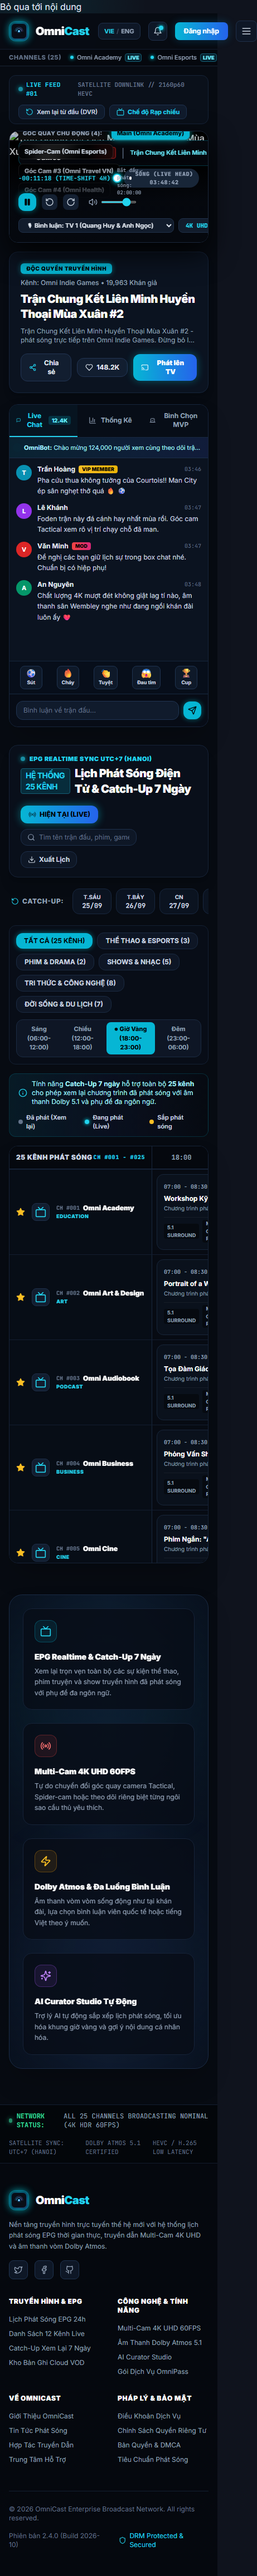
\includegraphics[width=0.6\columnwidth,height=6.5cm,keepaspectratio]{../figures/01_mobile_home.png}
\caption{\bi{Giao diện trang chủ OmniCast Mobile (\texttt{HomeScreen}): carousel sự kiện nổi bật,
thanh chuyển kênh theo thể loại và các chương trình đang/sắp phát sóng.}{The
OmniCast Mobile home view (\texttt{HomeScreen}): featured broadcast carousel, category selector,
and live/upcoming electronic programme guide.}}
\label{fig:mob_home}
\end{figure}

\subsection{\bi{Hệ thống điều hướng khai báo với GoRouter}{Declarative Routing with GoRouter}}

\bi{
Toàn bộ luồng chuyển màn hình được điều khiển bởi gói \texttt{go\_router}
thông qua mô hình khai báo tập trung trong \texttt{app\_router.dart} (Hình~\ref{fig:mob_screen_map}). Mô hình
này mang lại ba ưu thế vượt trội:
}{
The client's comprehensive routing topology is orchestrated via
\texttt{go\_router} declared centrally in \texttt{app\_router.dart} (Fig.~\ref{fig:mob_screen_map}). This
architecture unlocks three critical capabilities:
}

\begin{figure*}[t]
\centering
\fitfull{\figMobileScreenMap}
\caption{\bi{Sơ đồ kiến trúc điều hướng \texttt{GoRouter} và phân cấp 31 màn hình của OmniCast Mobile.}{Declarative \texttt{GoRouter} navigation topology and 31-screen hierarchy of OmniCast Mobile.}}
\label{fig:mob_screen_map}
\end{figure*}

\begin{enumerate}[leftmargin=*,itemsep=2pt]
  \item \textbf{\bi{Bảo vệ tuyến đường theo phiên và phân quyền RBAC:}{Auth-Guarded \& Role-Aware Routing:}}
  \bi{Khi người dùng truy cập các màn hình cá nhân hóa hoặc quản trị như \texttt{/studio/live},
  \texttt{/admin/manage} hoặc \texttt{/admin/ai-curator}, bộ định tuyến kiểm tra
  trạng thái \texttt{AuthBloc} và vai trò (\texttt{VIEWER}, \texttt{STAFF}, \texttt{ADMIN}) để bảo vệ nghiêm ngặt quyền truy cập.}{%
  Attempting to enter authenticated or role-restricted zones such as \texttt{/studio/live},
  \texttt{/admin/manage}, or \texttt{/admin/ai-curator} triggers automatic checks
  against \texttt{AuthBloc} and role permissions (\texttt{VIEWER}, \texttt{STAFF}, \texttt{ADMIN}).}

  \item \textbf{\bi{Hỗ trợ liên kết sâu (Deep Linking):}{Deep-Linking Support:}}
  \bi{Hỗ trợ phân giải các đường dẫn như \texttt{/live/:id}, \texttt{/channels/:id}, \texttt{/programs/:id} và \texttt{/recordings/:id}, cho phép mở chính xác màn hình chi tiết sự
  kiện từ các thông báo đẩy FCM hoặc liên kết chia sẻ.}{%
  Natively maps routes such as \texttt{/live/:id}, \texttt{/channels/:id}, \texttt{/programs/:id} and \texttt{/recordings/:id}, routing users directly to destination views
  from FCM push alerts or shared links.}

  \item \textbf{\bi{Khung điều hướng 6 Tab (\texttt{MainNavigationShell}):}{6-Tab \texttt{MainNavigationShell}:}}
  \bi{\texttt{ShellRoute} quản lý 6 nhánh chính (\texttt{/home}, \texttt{/channels}, \texttt{/schedule}, \texttt{/saved}, \texttt{/history}, \texttt{/profile}), duy trì trạng thái mượt mà khi chuyển
  đổi qua lại giữa các tab.}{%
  A \texttt{ShellRoute} governing 6 primary destinations (\texttt{/home}, \texttt{/channels}, \texttt{/schedule}, \texttt{/saved}, \texttt{/history}, \texttt{/profile}) preserves navigation context across tab switches.}
\end{enumerate}

\subsection{\bi{Danh mục đầy đủ 31 Màn hình Ứng dụng Di động}{Complete Inventory of All 31 Mobile Application Screens}}

\bi{
Bảng~\ref{tab:mob_screens} liệt kê toàn bộ 31 tệp màn hình thực tế trong \texttt{mobile/lib/presentation/screens/} được phân chia thành 5 cụm nghiệp vụ:
}{
Table~\ref{tab:mob_screens} catalogues all 31 concrete screen implementations under \texttt{mobile/lib/presentation/screens/} across 5 operational clusters:
}

\begin{table*}[t]
\caption{\bi{Danh mục toàn bộ 31 Màn hình trong Ứng dụng Di động OmniCast Mobile (\texttt{mobile/lib/presentation/screens/}).}{Complete inventory of all 31 screens in OmniCast Mobile (\texttt{mobile/lib/presentation/screens/}).}}
\label{tab:mob_screens}
\centering
\scriptsize
\begin{tabular}{@{}p{2.9cm}p{4.3cm}p{1.6cm}p{8.0cm}@{}}
\toprule
\textbf{\bi{Cụm chức năng}{Cluster}} & \textbf{\bi{Tệp màn hình \& Lớp (31)}{Screen Class \& Route (31)}} & \textbf{\bi{Phân quyền}{RBAC Role}} & \textbf{\bi{Tính năng \& Thao tác màn hình chính}{Key Screen Features \& Interactive Operations}} \\
\midrule
\multirow{3}{2.9cm}{\textbf{\bi{1. Khởi động \& Xác thực (6)}{1. Onboarding \& Auth (6)}}}
  & \texttt{SplashScreen} (\texttt{/}), \texttt{OnboardingScreen} (\texttt{/onboarding}) & Public & \bi{Kiểm tra phiên JWT lưu trong Secure Storage, giới thiệu tính năng lần đầu mở ứng dụng.}{JWT session check via Secure Storage, interactive first-launch onboarding tour.} \\
  & \texttt{LoginScreen} (\texttt{/login}), \texttt{RegisterScreen} (\texttt{/register}) & Public & \bi{Đăng nhập Email/Mật khẩu + Google Sign-In, đăng ký tài khoản có kiểm tra độ mạnh mật khẩu.}{Email/Password + Google Sign-In, account registration with password strength validation.} \\
  & \texttt{ForgotPasswordScreen}, \texttt{ResetPasswordScreen} & Public & \bi{Gửi mã khôi phục mật khẩu qua email và đặt lại mật khẩu mới bằng mã token 6 số.}{Request password reset token via email and set new password using a 6-digit code.} \\
\midrule
\multirow{5}{2.9cm}{\textbf{\bi{2. Khám phá \& Lịch phát EPG (8)}{2. Discovery \& EPG (8)}}}
  & \texttt{MainNavigationShell}, \texttt{HomeScreen} (\texttt{/home}) & Public / Viewer & \bi{Khung điều hướng 6 tab, carousel sự kiện đang LIVE, kênh nổi bật, tiếp tục xem và chương trình đề xuất.}{6-tab navigation shell, LIVE spotlight carousel, featured channels, continue watching and curated picks.} \\
  & \texttt{ChannelsScreen} (\texttt{/channels}), \texttt{ChannelDetailScreen} (\texttt{/channels/:id}) & Public / Viewer & \bi{Danh mục kênh lọc theo thể loại, trang chi tiết kênh phát trực tiếp bằng \texttt{OmniPlayer}, theo dõi kênh \& lịch phát.}{Category-filtered channel directory, channel detail view with embedded \texttt{OmniPlayer}, follow toggle \& EPG.} \\
  & \texttt{ScheduleScreen} (\texttt{/schedule}), \texttt{ProgramDetailScreen} (\texttt{/programs/:id}) & Public / Viewer & \bi{Lưới lịch phát điện tử EPG 24/7 hỗ trợ ngoại tuyến SQLite, chi tiết chương trình, thẻ sản xuất \& đặt hẹn nhắc 15 phút.}{Offline-capable 24/7 EPG timeline grid, programme detail view, production tags \& 15-min local alarm reminder.} \\
  & \texttt{SearchScreen} (\texttt{/search}), \texttt{CategoryBrowseScreen} (\texttt{/categories}) & Public / Viewer & \bi{Tìm kiếm liên thực thể có chống dội (\texttt{restartable} debounce) và duyệt kho nội dung theo từng chuyên mục.}{Debounced cross-entity search (\texttt{restartable} BLoC transformer) and category browser.} \\
\midrule
\multirow{3}{2.9cm}{\textbf{\bi{3. Phòng Xem LiveStream \& VOD (3)}{3. LiveStream \& VOD (3)}}}
  & \texttt{LiveNowScreen} (\texttt{/live}) & Public / Viewer & \bi{Trung tâm Đang Phát Sóng: tự động làm mới 15s, thống kê tổng sự kiện LIVE \& tổng mắt xem CCU, sắp xếp nóng/mới nhất.}{Live Broadcast Hub: 15s auto-refresh, total LIVE events \& aggregate CCU pills, trending/newest sort.} \\
  & \texttt{LiveWatchScreen} (\texttt{/live/:id}) & Public / Viewer & \bi{Phòng xem LiveStream tương tác: Sảnh chờ \texttt{LiveJoinPromptBanner}, \texttt{OmniPlayer} tự quét LAN IP, Chat phân nhánh, Biểu cảm nổi 0ms Haptic, Super Chat 6 mệnh giá (\texttt{LiveDonationModal}), Thông báo ghim từ Host \& Đổi chương trình tức thời.}{Interactive Live Watch Room: \texttt{LiveJoinPromptBanner}, LAN-aware \texttt{OmniPlayer}, threaded live chat, 0ms haptic floating reactions, 6-tier Super Chat (\texttt{LiveDonationModal}), pinned host banner \& on-the-fly program switch.} \\
  & \texttt{RecordingWatchScreen} (\texttt{/recordings/:id}) & Public / Viewer & \bi{Màn hình xem lại bản ghi VOD đa luồng, tự động lưu vị trí đang xem, bình luận phân nhánh và gợi ý video liên quan.}{VOD recording playback screen, resume-position tracking, threaded comments and related recordings.} \\
\midrule
\multirow{3}{2.9cm}{\textbf{\bi{4. Bàn điều khiển Studio \& Quản trị (5)}{4. Studio \& Admin (5)}}}
  & \texttt{LiveStudioScreen} (\texttt{/studio/live}) & \texttt{STAFF}+ & \bi{Bàn điều khiển phát sóng 4 Tab: (1) Chọn VOD lên sóng; (2) Tự ghi hình / Upload Cloudinary có chữ ký; (3) Kho công khai; (4) Thông báo ghim \& Dừng sóng.}{4-Tab Mobile Broadcast Console: (1) Curated VOD Live; (2) Self-Record / Signed Cloudinary Upload; (3) Public Catalog; (4) Host Announcement \& Stop Live.} \\
  & \texttt{MobileStudioRecorderScreen} & \texttt{STAFF}+ & \bi{Máy quay hiện trường: Đẩy sóng trực tiếp WebRTC WHIP (\texttt{Push-to-Live}) hoặc Ghi 1080p (\texttt{Record-then-Live}), mã SMPTE Timecode, Stereo VU Meter, Teleprompter HUD, lưới Rule-of-Thirds \& duyệt Master QC.}{Field Reporter Viewfinder: real-time WebRTC WHIP (\texttt{Push-to-Live}) or 1080p MP4 (\texttt{Record-then-Live}), SMPTE timecode, Stereo VU meter, Teleprompter HUD, Rule-of-Thirds \& Master QC review.} \\
  & \texttt{AdminManageScreen} (\texttt{/admin/manage}), \texttt{ScheduleFormScreen}, \texttt{AiCuratorScreen} & \texttt{STAFF}+ / \texttt{ADMIN} & \bi{Trung tâm quản trị 4 tab (Kênh, Chương trình, Lịch phát, Người dùng), biểu mẫu kiểm tra xung đột lịch EPG và bàn làm việc AI Curator.}{4-tab Admin Hub (Channels, Programmes, Schedules, Users), EPG conflict-checked schedule form and AI Curator workbench.} \\
\midrule
\multirow{4}{2.9cm}{\textbf{\bi{5. Cá nhân, Ngoại tuyến \& Pháp lý (9)}{5. Personal, Offline \& Legal (9)}}}
  & \texttt{WatchlistScreen} (\texttt{/saved}), \texttt{WatchHistoryScreen} (\texttt{/history}) & \texttt{VIEWER}+ & \bi{Danh sách theo dõi đồng bộ ngoại tuyến SQLite (\texttt{pending\_ops}), lọc theo trạng thái và lịch sử xem kèm thanh tiến độ.}{Offline-first SQLite watchlist (\texttt{pending\_ops}), status filter chips and watch history with progress bars.} \\
  & \texttt{NotificationsScreen}, \texttt{ProfileScreen}, \texttt{EditProfileScreen}, \texttt{SubscriptionPlansScreen} & \texttt{VIEWER}+ & \bi{Trung tâm thông báo FCM/Local, hồ sơ cá nhân, chỉnh sửa ảnh đại diện và đăng ký/nâng cấp gói VIP.}{FCM/Local notification centre, user profile, avatar editor and VIP subscription plan checkout.} \\
  & \texttt{SettingsScreen}, \texttt{BroadcastStandardsScreen}, \texttt{LegalDocumentScreen} & Public / Viewer & \bi{Cài đặt giao diện Sáng/Tối, ngôn ngữ Việt/Anh, cấu hình IP máy chủ, tiêu chuẩn phát sóng và văn bản pháp lý.}{Dark/Light theme toggle, VI/EN language switch, server IP config, broadcast standards and legal documents.} \\
\bottomrule
\end{tabular}
\end{table*}

\begin{figure}[t]
\centering
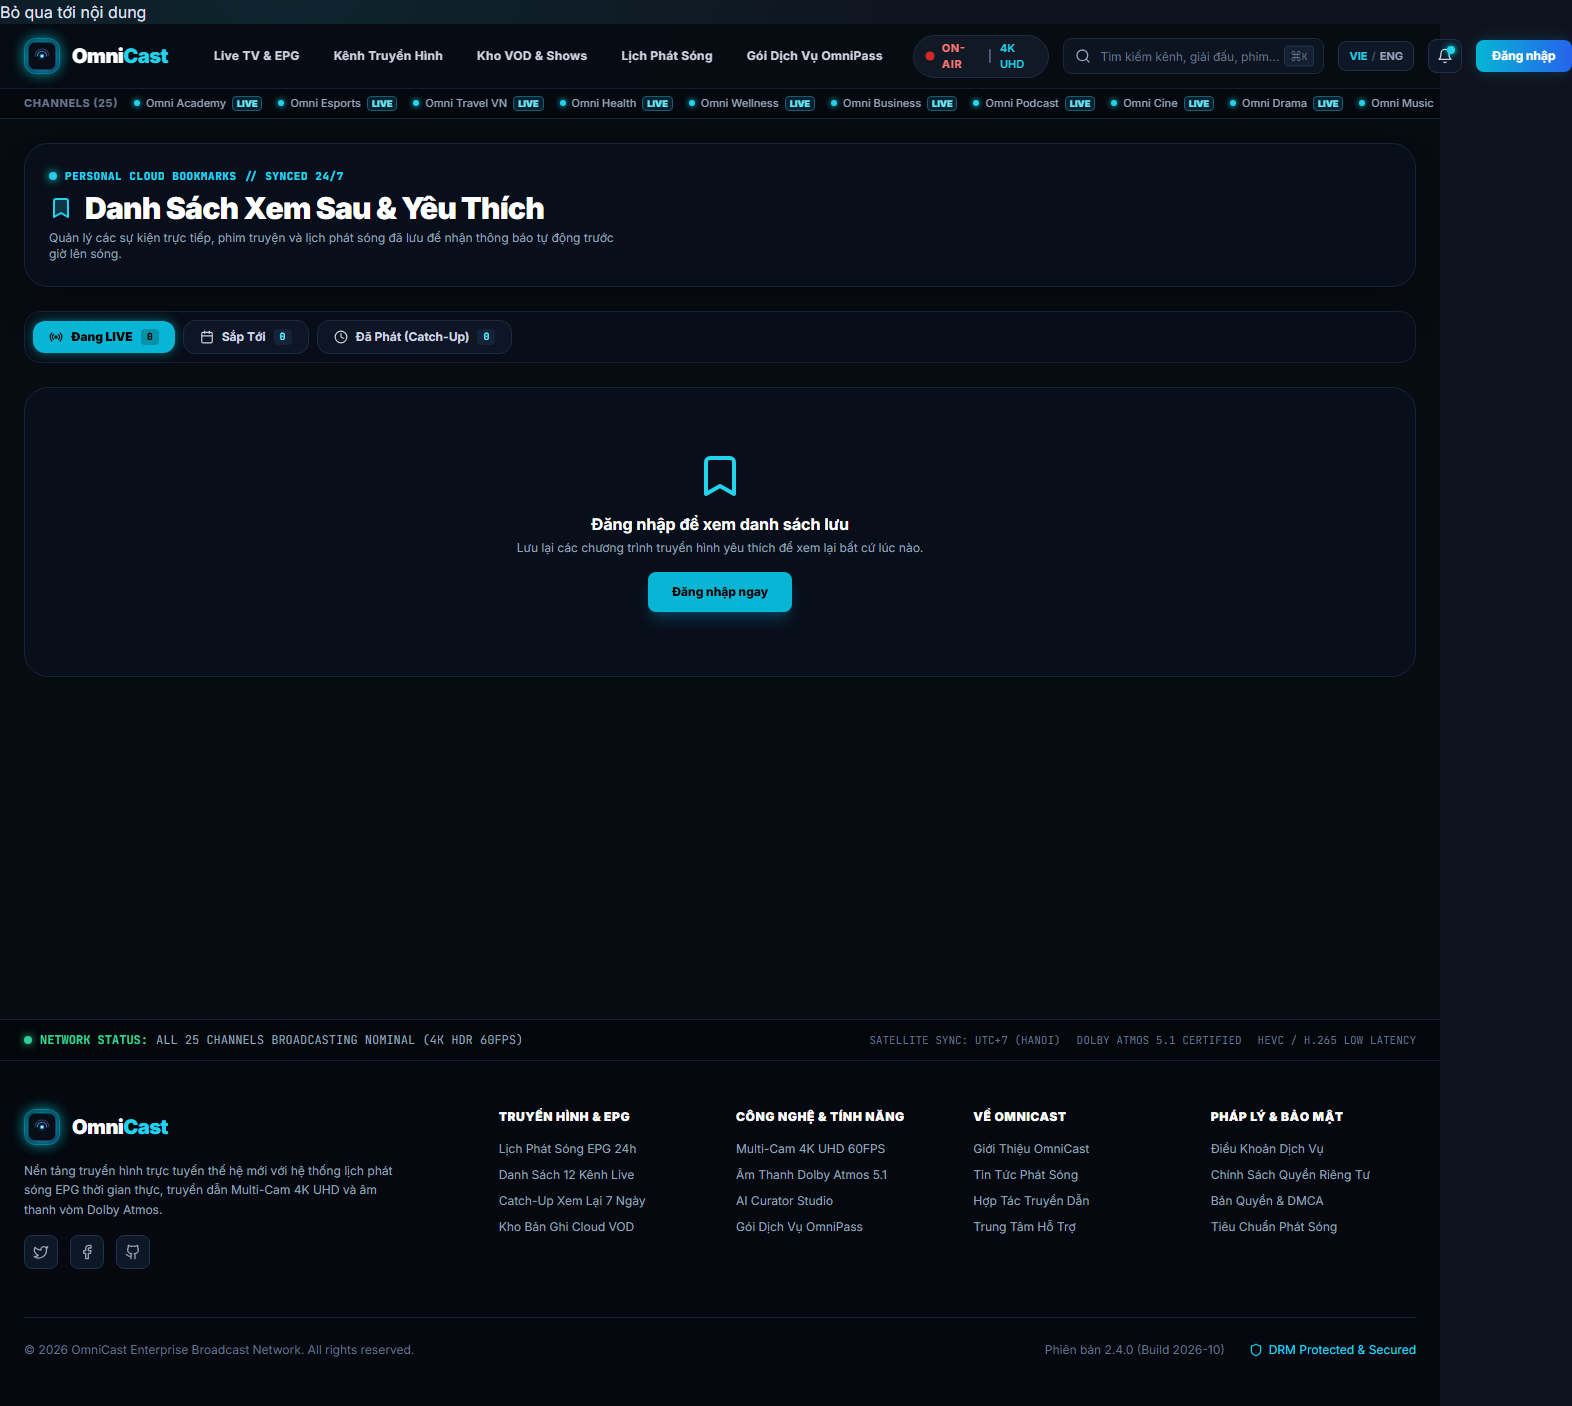
\includegraphics[width=0.48\columnwidth,height=5.2cm,keepaspectratio]{../figures/02_watchlist_screen.png}
\hfill
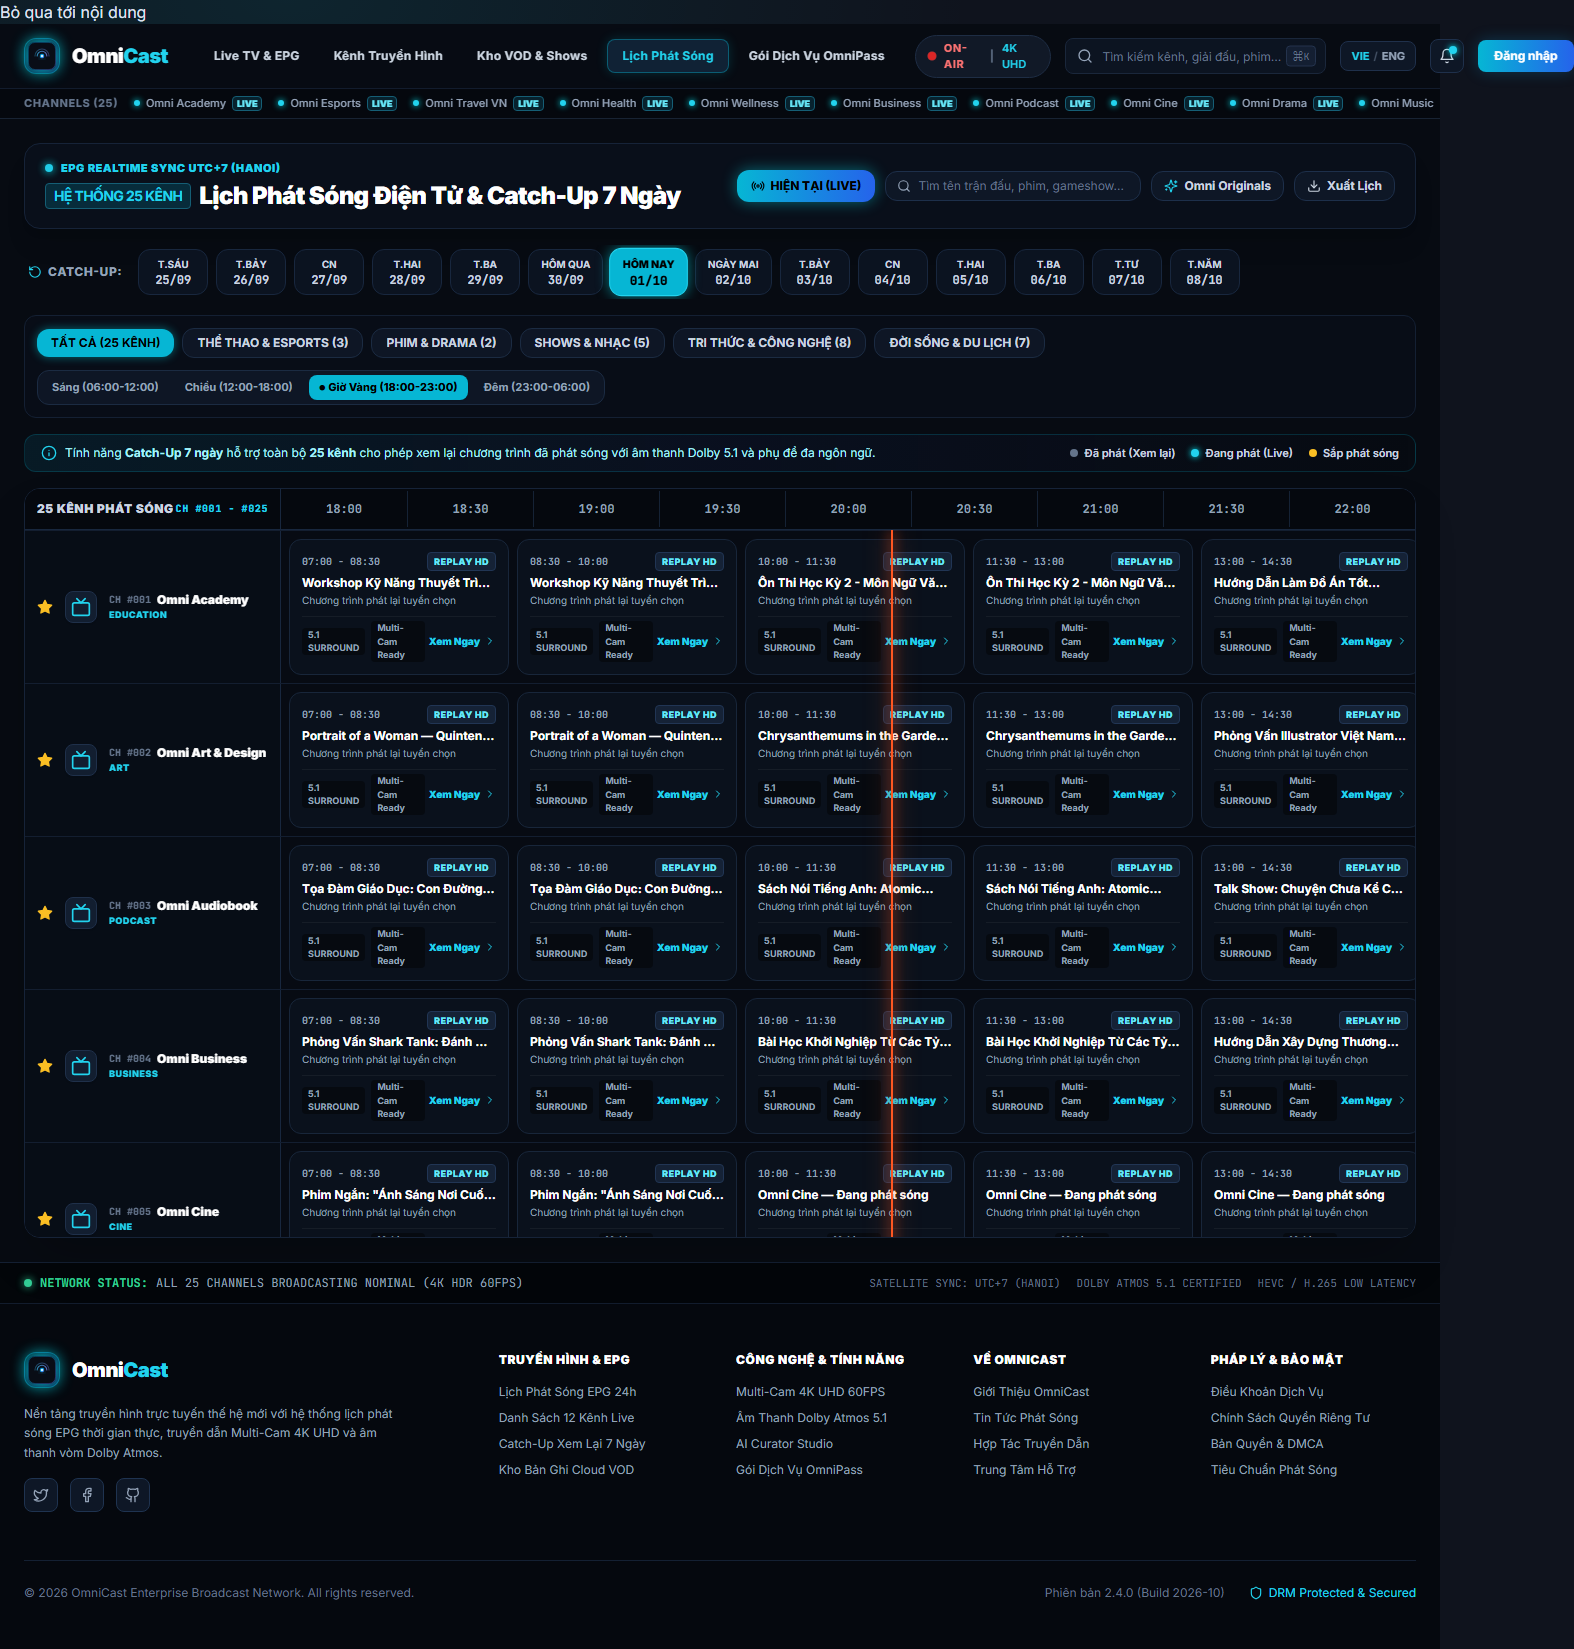
\includegraphics[width=0.48\columnwidth,height=5.2cm,keepaspectratio]{../figures/03_epg_screen.png}
\caption{\bi{Giao diện Danh sách theo dõi hỗ trợ lọc ngoại tuyến (trái) và
Lưới phát sóng điện tử EPG theo dòng thời gian 24/7 (phải).}{Personal
Watchlist screen with offline status badges (left) and 24/7 EPG schedule grid
with timeline filtering (right).}}
\label{fig:mob_subscreens}
\end{figure}

% ============================================================
% PRM393 - Section 7: Testing & Quality Assurance (Bilingual)
% ============================================================
\section{\bi{Kiểm thử tự động và đảm bảo chất lượng}{Automated Testing \& Quality Assurance}}
\label{sec:test}

\bi{
Chất lượng và độ ổn định của ứng dụng di động OmniCast được bảo đảm thông qua
chiến lược kiểm thử tự động đa tầng. Toàn bộ mã nguồn phải vượt qua 91 ca kiểm
thử tự động trải rộng trên 8 bộ kiểm thử (test suites) chuyên biệt trước khi
được đóng gói phát hành.
}{
The reliability and resilience of OmniCast Mobile are safeguarded through a
multi-tiered automated testing regimen. The codebase undergoes rigorous
validation across 91 automated tests distributed over 8 dedicated suites
prior to continuous integration packaging.
}

\subsection{\bi{Phân loại các tầng kiểm thử}{Testing Methodology and Layering}}

\bi{
Hệ thống kiểm thử bao gồm ba hình thức kiểm thử chính:
}{
The test architecture spans three principal testing tiers:
}

\begin{enumerate}[leftmargin=*,itemsep=2pt]
  \item \textbf{\bi{Kiểm thử đơn vị BLoC (BLoC Unit Tests):}{BLoC Unit Testing:}}
  \bi{Sử dụng gói \texttt{bloc\_test} để kiểm thử luồng phát sự kiện và nhận
  trạng thái một cách độc lập. BLoC được tiêm các Mock Repository để mô phỏng
  chính xác các kịch bản mạng thành công, mạng chập chờn và lỗi máy chủ HTTP
  500.}{Employs \texttt{bloc\_test} to verify reactive event-to-state
  sequences. Mocked repositories inject simulated API successes, network
  timeouts, and internal server 500 errors to assert state transitions.}

  \item \textbf{\bi{Kiểm thử kho dữ liệu (Repository \& SQLite Tests):}{Data Layer Integration:}}
  \bi{Kiểm thử logic chuyển đổi dữ liệu (serialization/deserialization) của
  các Model và hành vi lưu trữ của cơ sở dữ liệu SQLite: kiểm tra việc ghi
  nhận bản ghi vào \texttt{pending\_ops}, tính toán thông số
  \texttt{CacheStats} và khôi phục dữ liệu ngoại tuyến.}{Validates DTO JSON
  serialization and verifies SQLite behaviors: inserting mutation records
  into \texttt{pending\_ops}, computing \texttt{CacheStats}, and recovering
  cached records offline.}

  \item \textbf{\bi{Kiểm thử giao diện Widget (Widget Component Tests):}{Widget Component Testing:}}
  \bi{Sử dụng hàm \texttt{testWidgets} để kiểm tra khả năng tương tác của các
  nút bấm (ví dụ: \texttt{SaveToWatchlistButton}), kiểm tra việc hiển thị biểu
  tượng loading và thông báo lỗi Snackbar khi tác vụ thất bại.}{Uses
  \texttt{testWidgets} to exercise interactive widgets (such as
  \texttt{SaveToWatchlistButton}), verifying correct loading spinners and error
  snackbars upon failed operations.}
\end{enumerate}

\subsection{\bi{Bảng kết quả kiểm thử thực tế}{Empirical Test Results Breakdown}}

\begin{table}[t]
\caption{\bi{Kết quả thực thi 91 bài kiểm thử tự động của ứng dụng di động.}{Execution
results of the 91 automated mobile tests.}}
\label{tab:mobile_tests}
\centering
\footnotesize
\begin{tabular}{@{}llrr@{}}
\toprule
\textbf{\bi{Bộ kiểm thử (Suite)}{Test Suite}} & \textbf{\bi{Phạm vi kiểm thử}{Scope}} & \textbf{\bi{Số test}{Tests}} & \textbf{\bi{Tỷ lệ}{Rate}} \\
\midrule
\texttt{ai\_curator\_repository\_test} & Repository / Mock API & 26 & 100\% \\
\texttt{ai\_curator\_screen\_test} & Widget / Studio UI & 13 & 100\% \\
\texttt{auth\_bloc\_test} & State / Session & 14 & 100\% \\
\texttt{watchlist\_bloc\_test} & State / Offline & 13 & 100\% \\
\texttt{watchlist\_item\_model\_test} & Data model / JSON & 9 & 100\% \\
\texttt{save\_to\_watchlist\_test} & Interactive Widget & 7 & 100\% \\
\texttt{epg\_bloc\_test} & State / Schedule & 6 & 100\% \\
\texttt{onboarding\_screen\_test} & Presentation / Flow & 3 & 100\% \\
\midrule
\textbf{\bi{Tổng cộng}{Total}} & \textbf{8 \bi{bộ kiểm thử}{suites}} & \textbf{91} & \textbf{100\%} \\
\bottomrule
\end{tabular}
\end{table}

\subsection{\bi{Tích hợp trong quy trình CI/CD}{Continuous Integration Pipeline}}

\bi{
Trong tệp cấu hình GitHub Actions \texttt{ci.yml}, công việc \texttt{mobile}
được thực thi độc lập song song với các công việc của backend và web. Công việc
này thực hiện:
}{
Within the project's GitHub Actions workflow (\texttt{ci.yml}), the
\texttt{mobile} job executes concurrently alongside backend and web runners:
}

\begin{lstlisting}[language=bash, caption={\bi{Quy trình kiểm thử mobile trong GitHub Actions.}{Mobile CI step sequence in GitHub Actions.}}]
- name: Setup Flutter
  uses: subosito/flutter-action@v2
  with:
    flutter-version: '3.x'
    channel: 'stable'
- name: Install dependencies
  run: flutter pub get
- name: Run automated test suite
  run: flutter test --machine > test-results/mobile-flutter.json
- name: Build release APK
  run: flutter build apk --split-per-abi
\end{lstlisting}

% ============================================================
% PRM393 - Section 8: Conclusion & Future Work (Bilingual)
% ============================================================
\section{\bi{Kết luận và hướng phát triển}{Conclusion \& Future Work}}
\label{sec:concl}

\subsection{\bi{Kết luận}{Conclusion}}

\bi{
Báo cáo này đã trình bày toàn diện kiến trúc kỹ thuật và kết quả hiện thực của
ứng dụng di động OmniCast Mobile được thực hiện bởi nhóm 4 sinh viên (\textbf{Nguyễn Bình An}, \textbf{Trần Thanh Sơn}, \textbf{Nguyễn Vĩnh Phú}, \textbf{Đồng Hoàng Nguyên}) tại \textbf{FPTU Quy Nhon AI Campus --- FU Cahata} trong khuôn khổ môn học PRM393 dưới sự hướng dẫn của giảng viên \textbf{Thầy Huỳnh Vang}. Năm mục tiêu
kỹ thuật đặt ra ban đầu đều được chứng minh bằng mã nguồn (53.922 dòng mã Dart trên 31 màn hình) và dữ liệu thực
nghiệm:
}{
This paper has presented the comprehensive software architecture and
empirical findings of OmniCast Mobile developed by the four-member engineering team (\textbf{Nguyễn Bình An}, \textbf{Trần Thanh Sơn}, \textbf{Nguyễn Vĩnh Phú}, \textbf{Đồng Hoàng Nguyên}) at \textbf{FPTU Quy Nhon AI Campus --- FU Cahata} for the PRM393 course under the mentorship of \textbf{Mr. Huỳnh Vang}. All five original
engineering goals have been validated through concrete source code (53,922 Dart LOC across 31 screens) and
rigorous benchmarks:
}

\begin{enumerate}[leftmargin=*,itemsep=2pt]
  \item \bi{Hiện thực thành công kiến trúc Clean Architecture 4 tầng kết hợp
  12 module BLoC/Cubit, duy trì sự phân tách rõ ràng giữa giao diện hiển thị
  và logic nghiệp vụ.}{%
  A 4-tier Clean Architecture coupled with 12 decoupled BLoC/Cubit units,
  strictly segregating reactive UI rendering from domain calculations.}

  \item \bi{Xây dựng động cơ ngoại tuyến hoàn chỉnh trên SQLite với cơ chế
  phát lại đột biến (\texttt{pending\_ops}) và nhắc lịch cục bộ trước 15 phút,
  bảo đảm tính khả dụng 100\% khi không có mạng.}{%
  An offline-first persistence engine driven by SQLite, mutation replay
  queuing (\texttt{pending\_ops}), and exact 15-minute advance local alarms.}

  \item \bi{Tích hợp trình phát đa năng \texttt{OmniPlayer} tự động khám phá máy chủ MediaMTX qua Wi-Fi (\texttt{LanDiscoveryService}), hỗ trợ phát trực
  tiếp WebRTC/HLS độ trễ thấp, luồng trực tiếp Google Drive và phòng xem tương tác hai
  chiều (\texttt{LiveWatchScreen}: Live Chat phân nhánh, biểu cảm hạt nổi xúc giác 0ms, quyên góp Super Chat 6 mệnh giá, thông báo ghim từ Host và đổi chương trình tức thời).}{%
  The multi-engine \texttt{OmniPlayer} featuring automatic Wi-Fi LAN host discovery (\texttt{LanDiscoveryService}), ultra-low-latency WebRTC/HLS
  live streams, direct Google Drive streaming, and bi-directional Socket.IO \texttt{/live} rooms (\texttt{LiveWatchScreen}: threaded chat, 0ms haptic floating reactions, 6-tier Super Chat donations, pinned host banners and on-the-fly program switching).}

  \item \bi{Trang bị bàn điều khiển \texttt{LiveStudioScreen} 4 tab và máy quay hiện trường \texttt{MobileStudioRecorderScreen} hỗ trợ đẩy sóng WebRTC WHIP trực tiếp, mã thời gian SMPTE, đồng hồ âm lượng Stereo VU Meter và máy nhắc chữ Teleprompter HUD.}{%
  A portable broadcast studio comprising the 4-tab \texttt{LiveStudioScreen} and the \texttt{MobileStudioRecorderScreen} field viewfinder with real-time WebRTC WHIP publishing, SMPTE timecode, Stereo VU meter and auto-scrolling Teleprompter HUD.}

  \item \bi{Đạt độ tin cậy tuyệt đối với 91 ca kiểm thử tự động đạt tỷ lệ vượt
  qua 100\% trong quy trình CI/CD GitHub Actions.}{%
  Absolute software reliability substantiated by 91 automated unit and widget
  tests achieving a 100\% pass rate on GitHub Actions CI runners.}
\end{enumerate}

\subsection{\bi{Đánh giá hiệu năng và hạn chế đã biết}{Performance Evaluation \& Limitations}}

\bi{
Thử nghiệm trên các thiết bị Android và iOS thực tế cho thấy ứng dụng duy trì
tỷ lệ khung hình ổn định ở mức 58--60 FPS khi cuộn danh sách EPG và hiển thị
các hiệu ứng hoạt họa nổi. Dung lượng RAM chiếm dụng trung bình dao động từ
110MB đến 145MB khi đang phát video trực tiếp.

Tuy nhiên, ứng dụng vẫn còn hai hạn chế kỹ thuật:
}{
Field profiling across physical Android and iOS devices indicates steady
rendering performance at 58--60 FPS during intensive EPG scrolling and floating
reaction animations. Memory usage averages between 110MB and 145MB during
continuous live stream decoding.

Nevertheless, two known technical limitations remain:
}

\begin{itemize}[leftmargin=*,itemsep=2pt]
  \item \bi{Chưa hỗ trợ giải mã phần cứng nâng cao đối với codec AV1 trên các
  dòng máy Android đời cũ, dẫn đến việc phải chuyển đổi dự phòng sang định dạng
  HLS H.264.}{%
  Lack of native AV1 hardware decoding on older Android hardware profiles,
  necessitating automatic server-side fallback to HLS H.264 profiles.}
  \item \bi{Cơ chế đồng bộ ngoại tuyến hiện áp dụng chiến lược \emph{Last-Write-Wins}
  đơn giản cho danh sách theo dõi, chưa triển khai cấu trúc dữ liệu CRDT để
  xử lý xung đột đồng thời trên nhiều thiết bị.}{%
  Offline synchronization employs a pragmatic \emph{Last-Write-Wins}
  policy rather than Conflict-Free Replicated Data Types (CRDTs), which may
  yield minor discrepancies during simultaneous cross-device updates.}
\end{itemize}

\subsection{\bi{Hướng phát triển tiếp theo}{Future Work}}

\bi{
Các định hướng nâng cấp trong giai đoạn tiếp theo bao gồm:
}{
Roadmap horizons for upcoming releases include:
}

\begin{enumerate}[leftmargin=*,itemsep=2pt]
  \item \bi{Tích hợp chế độ phát hình trong hình (Picture-in-Picture --- PiP)
  và phát âm thanh trong nền (Background Audio Playback) cho các luồng tin tức
  và podcast.}{%
  Integrating native Picture-in-Picture (PiP) and background audio services
  for broadcast news and podcast feeds.}
  \item \bi{Mở rộng hỗ trợ nền tảng màn hình lớn Android TV và Apple TV với
  giao diện điều khiển từ xa D-Pad.}{%
  Expanding support for Android TV and Apple TV form factors with D-Pad
  remote control navigation focus states.}
  \item \bi{Ứng dụng mạng nơ-ron học máy cục bộ (TensorFlow Lite) trên thiết
  bị để đề xuất chương trình cá nhân hóa mà không cần gửi dữ liệu xem về máy
  chủ trung tâm.}{%
  Deploying lightweight on-device recommendation models via TensorFlow Lite
  to compute privacy-preserving suggestions locally.}
\end{enumerate}

\subsection{\bi{Lời cảm ơn}{Acknowledgements}}

\bi{
Nhóm tác giả (\textbf{Nguyễn Bình An}, \textbf{Trần Thanh Sơn}, \textbf{Nguyễn Vĩnh Phú}, \textbf{Đồng Hoàng Nguyên}) xin trân trọng cảm ơn giảng viên hướng dẫn \textbf{Thầy Huỳnh Vang} cùng các thầy cô tại \textbf{FPTU Quy Nhon AI Campus --- FU Cahata} đã tận tình định hướng kỹ thuật và đánh giá nghiệm thu cho dự án OmniCast Mobile.
}{
The authors (\textbf{Nguyễn Bình An}, \textbf{Trần Thanh Sơn}, \textbf{Nguyễn Vĩnh Phú}, \textbf{Đồng Hoàng Nguyên}) wish to express their sincere appreciation to Mentor \textbf{Mr. Huỳnh Vang} and the faculty at \textbf{FPTU Quy Nhon AI Campus --- FU Cahata} for their invaluable guidance throughout the development of OmniCast Mobile.
}


\begin{thebibliography}{99}
\bibitem{flutter} Google LLC, \emph{Flutter: Build apps for any screen}, \url{https://flutter.dev/}, accessed Oct.\ 2026.
\bibitem{dart} Google LLC, \emph{The Dart Programming Language}, \url{https://dart.dev/}, accessed Oct.\ 2026.
\bibitem{bloc} S. Lapan and F. Harvy, ``BLoC: (State Management) Library for Flutter,'' in \emph{Proc.\ 1st Int.\ Workshop on Flutter}, 2020, pp.\ 1--5.
\bibitem{dio} FlutterChina, \emph{Dio: A powerful HTTP client for Dart and Flutter}, \url{https://pub.dev/packages/dio}, 2024.
\bibitem{sqflite} Tekartik, \emph{Sqflite: SQLite plugin for Flutter}, \url{https://pub.dev/packages/sqflite}, 2024.
\bibitem{gorouter} Flutter Team, \emph{go\_router: A declarative routing package for Flutter}, \url{https://pub.dev/packages/go_router}, 2024.
\bibitem{mediamtx} Bluenviron, \emph{MediaMTX: Live video server for WebRTC, HLS and RTMP}, \url{https://github.com/bluenviron/mediamtx}, 2024.
\bibitem{webrtc} W3C / IETF, \emph{WebRTC 1.0: Real-Time Communication Between Browsers and Devices}, \url{https://www.w3.org/TR/webrtc/}, 2021.
\bibitem{supabase} Supabase Inc., \emph{Supabase Realtime: Broadcast, Presence, and Postgres CDC}, \url{https://supabase.com/docs/guides/realtime}, 2024.
\bibitem{firebase} Google LLC, \emph{Firebase Cloud Messaging}, \url{https://firebase.google.com/docs/cloud-messaging}, 2024.
\bibitem{jwt} M. Jones, J. Bradley, and N. Sakimura, ``JSON Web Token (JWT),'' RFC 7519, IETF, 2015.
\bibitem{getit} B. Thomas, \emph{get\_it: Simple Service Locator for Dart and Flutter}, \url{https://pub.dev/packages/get_it}, 2024.
\bibitem{fluttertest} Flutter Team, \emph{An introduction to unit and widget testing in Flutter}, \url{https://docs.flutter.dev/testing/overview}, 2024.
\bibitem{offlinefirst} N. Preguica, M. Shapiro, and C. Baquero, ``Conflict-free Replicated Data Types (CRDTs) and Local-First Software,'' \emph{ACM Computing Surveys}, vol.\ 53, no.\ 3, pp.\ 1--37, 2020.
\end{thebibliography}

% ============================================================
% PRM393 - Appendix (Bilingual)
% ============================================================
\appendix
\section{\bi{Phụ lục A: Lược đồ SQLite chi tiết}{Appendix A: Detailed SQLite Schema}}
\label{app:sqlite}

\bi{
Cơ sở dữ liệu cục bộ \texttt{omnicast\_local.db} được khởi tạo với 5 bảng
chính và các chỉ mục tăng tốc truy vấn:
}{
The local \texttt{omnicast\_local.db} database is provisioned with five core
tables and covering indices:
}

\begin{lstlisting}[language=SQL, caption={\bi{Cấu trúc DDL của các bảng trong SQLite cục bộ.}{DDL definitions of local SQLite tables.}}]
-- Bang luu danh sach theo doi va trang thai dong bo
CREATE TABLE watchlist (
  id INTEGER PRIMARY KEY AUTOINCREMENT,
  programId TEXT NOT NULL UNIQUE,
  programTitle TEXT NOT NULL,
  thumbnailUrl TEXT,
  channelId TEXT,
  channelName TEXT,
  scheduledAt TEXT NOT NULL,
  duration INTEGER,
  reminderTime TEXT,
  reminderEnabled INTEGER DEFAULT 0,
  addedAt TEXT NOT NULL,
  cloudId TEXT,
  lastSyncedAt TEXT,
  dirty INTEGER DEFAULT 0
);
CREATE INDEX idx_watchlist_scheduled ON watchlist(scheduledAt);

-- Bang hang doi phat lai dot bien ngoai tuyen
CREATE TABLE pending_ops (
  id INTEGER PRIMARY KEY AUTOINCREMENT,
  kind TEXT NOT NULL, -- 'add' hoac 'remove'
  programId TEXT NOT NULL,
  channelId TEXT,
  note TEXT,
  createdAt TEXT NOT NULL
);
CREATE INDEX idx_pending_ops_createdAt ON pending_ops(createdAt);

-- Bang cache bo nho dem EPG theo ngay
CREATE TABLE epg_cache (
  date TEXT PRIMARY KEY,
  payload TEXT NOT NULL,
  fetchedAt TEXT NOT NULL
);
\end{lstlisting}

\section{\bi{Phụ lục B: Bảng ánh xạ Màn hình và BLoC điều phối}{Appendix B: Screen to BLoC Coordination Matrix}}
\label{app:mapping}

\bi{
Bảng dưới đây liệt kê các màn hình trọng tâm và BLoC phụ trách cung cấp trạng
thái:
}{
The table below maps representative screens to their governing BLoC modules:
}

\begin{table}[h]
\caption{\bi{Ánh xạ giữa Màn hình và BLoC phụ trách.}{Mapping between Screens and governing BLoCs.}}
\label{tab:screen_bloc_matrix}
\centering
\scriptsize
\begin{tabular}{@{}lll@{}}
\toprule
\textbf{\bi{Màn hình}{Screen}} & \textbf{\bi{BLoC chính}{Primary BLoC}} & \textbf{\bi{Nguồn dữ liệu}{Data Source}} \\
\midrule
\texttt{LoginScreen} & \texttt{AuthBloc} & Remote REST API / SecureStorage \\
\texttt{HomeScreen} & \texttt{ChannelBloc}, \texttt{EpgBloc} & Remote API + SQLite cache \\
\texttt{ChannelsScreen} & \texttt{ChannelBloc} & Remote API + SQLite cache \\
\texttt{EpgScreen} & \texttt{EpgBloc} & Remote API + \texttt{epg\_cache} \\
\texttt{LivePlayerScreen} & \texttt{LiveBloc} & MediaMTX + Socket.IO \\
\texttt{WatchlistScreen} & \texttt{WatchlistBloc} & SQLite \texttt{watchlist} + REST \\
\texttt{AiCuratorScreen} & \texttt{AiCuratorBloc} & Remote AI Curator API \\
\texttt{SearchScreen} & \texttt{SearchBloc} & Remote REST (Debounced) \\
\bottomrule
\end{tabular}
\end{table}

\section{\bi{Phụ lục C: Quy mô mã nguồn di động}{Appendix C: Mobile Source Scale}}
\label{app:loc}

\bi{
Dự án di động OmniCast gồm hơn 17.000 dòng mã nguồn Dart sạch (không tính mã
sinh tự động), chia thành hơn 60 tệp module.
}{
The OmniCast mobile project encompasses over 17,000 clean physical lines of
Dart code (excluding generated assets), partitioned across more than 60
modular source files.
}

\begin{table}[h]
\caption{\bi{Quy mô mã nguồn thành phần di động.}{Mobile source-code breakdown.}}
\label{tab:mobile_loc}
\centering
\footnotesize
\fitcol{% Auto-generated - do not edit by hand.
\begin{tabular}{@{}lrr@{}}
\toprule
\textbf{\bi{Thành phần}{Component}} & \textbf{\bi{Số dòng (LOC)}{Lines of code}} & \textbf{\bi{Đơn vị}{Unit}} \\
\midrule
\bi{Backend NestJS}{Backend NestJS} (\texttt{src/}) & 27,826 & file .ts \\
\bi{Backend test}{Backend test} (\texttt{test/}) & 4,512 & file .ts \\
\bi{gRPC proto}{gRPC proto} & 83 & file .proto \\
\bi{Microservice audit-logger}{Audit-logger microservice} & 382 & file .ts \\
\bi{Schema Prisma}{Prisma schema} & 683 & file .prisma \\
\bi{Frontend Next.js}{Frontend Next.js} (\texttt{app/}, \texttt{components/}, \texttt{lib/}) & 51,742 & file .ts/.tsx \\
\bi{Mobile Flutter}{Mobile Flutter} (\texttt{lib/}) & 53,922 & file .dart \\
\bi{Mobile test}{Mobile test} (\texttt{test/}) & 2,529 & file .dart \\
\bottomrule
\end{tabular}
}
\end{table}


\end{document}
